\chapter{Análise Bibliográfica sobre Análise e Descrição de Vídeo, por Gabriel RochaFontenele\label{chap:bibliometria:ngsylar}}

\section{Planejamento do estudo}

Com o crescimento da tecnologia e o desenvolvimento de algoritmos, ferramentas e técnicas para análise e reconhecimento de padrões, tornou-se possível a abertura de pesquisas para elaboração de técnicas de descrição de diversos tipos de mídia. Tais técnicas podem ter uma área muito abrangente de aplicações, como reconhecimento de padrões de fala, reconhecimento linguagem, escrita, descrição de imagens ou descrição de vídeos ou cenas em movimento.

Aprofundando-se mais especificamente na parte da análise e descrição de vídeos ou cenas em movimento, podem ser utilizados algoritmos específicos para certos tipos de vídeo dado um contexto ou mesmo inteligência artificial e aprendizado de máquina para descrever em tempo real uma variedade muito maior de cenas com conteúdos variados. Assim, o foco na pesquisa e elaboração de soluções para problemas nessa área podem trazer um grande impacto sobre aplicação de reconhecimento de eventos em vídeo, descrição de eventos em câmeras de segurança, classificação etária etc.

A respeito do tema, as perguntas que nortearam a pequisa bibliográfica foram:

\begin{itemize}

\item O que já foi produzido cientificamente a respeito do tema?
\item Quais são as técnicas mais empregadas em relação a análise e descrição de cenas em movimento?
\item Quais são os países com maior quantidade e relevância em termos de produção científica?

\end{itemize}


\subsection{Ferramentas de apoio}

Para auxiliar o processo de análise da pesquisa bibliográfica, foi utilizado o pacote \textbf{Bibliometrix} da linguagem \textbf{R} através da interface gráfica \textbf{Biblioshiny}.

\subsection{Limitações} 
O exercício relatado foi feito em uma semana, utilizando os resultados de busca na base de dados \textit{Web of Science} (WoS).

\section{Coleta de dados}
A coleta de dados feita usando a base de dados WoS no dia 8 de fevereiro de 2022, acessado por meio do \textit{Portal de Periódicos da CAPES}. Foram feitas buscas nas coleções \textit{Science Citation Index Expanded (SCI -EXPANDED)} e \textit{Social Sciences Citation Index (SSCI)}, o primeiro mais focado na área das ciências exatas e naturais e o segundo na área das ciências sociais. Os artigos presentes nas duas coleções mecionadas foram indexados a partir de 1945.

A seguinte \textit{query} de busca foi elaborada para realização da pesquisa:

\lstinputlisting[
    numbers=left,
    basicstyle=\normalsize\ttfamily,
    caption={Query de busca para Análise e Descrição de Vídeo},
    label=IAeDiscriminacaoQuery
]{experiments/ngsylar/PesqBibliogr/query.txt}

\subsection{Explicação para os termos de busca usados}
A busca consistiu na intersecção de termos essencialmente ligados ao tema e que pudessem prover um panorama geral sobre o tema atualmente.

Os termos \texttt{(algorit* or (artificial and intelligen*))} foram usados para receber o retorno das buscas apenas relacionados a área da computação.

Os termos \texttt{(video or scene)} foram usados para cobrir os objetos de estudo da pesquisa, em se tratando de vídeos ou cenas com movimento, seja em tela ou câmera.

Já \texttt{analysis and descript*} foram utilizados para enfatizar estudos que tratam especificamente de técnicas de análise e descrição dos objetos de estudo.

Por fim, tudos os termos após a conjunção \textit{not} tiveram o único objetivo excluir temas não ligados a proposta inicial da busca.

\subsection{Registros recuperados}
Os 775 registros obtidos como resultado da busca encontram-se em \url{https://github.com/jhcf/Comput-Experim-20212}, no diretório {experiments/ngsylar/PesqBibliogr/WoS775recs.txt}.

A exportação do registro, com 69342 linhas em formato de texto não formatado, foi feita a partir de 22 campos referentes a \textit{Autor, Título, Fonte, Resumo, Palavra-chave, Endereços, Referências citadas e uso} no WoS.

\subsection{Análise dos dados}
Inicialmente foi observado de forma rápida os títulos recuperados na primeira página da busca e em seguida os termos da query foram refinados para a versão mencionada.
Posteriormente, foi feita uma vistoria no grafo de redes de co-ocorrência para verificar o peso das palavras presentes nos resultados da busca, como pode ser visto na imagem \ref{fig:evol:anual:cotonet:ASADES@ngsylar}.

\begin{figure}[H]
    \centering
    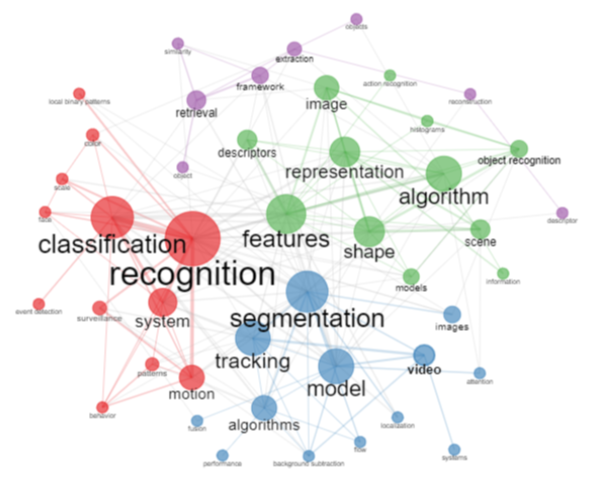
\includegraphics[width=1\textwidth]{experiments/ngsylar/PesqBibliogr/Imagens/ASADES-CoOccurrenceNetwork.png}
    \caption{Rede de Co-ocorrências de maior peso no dataset ASADES@ngsylar.}
    \label{fig:evol:anual:cotonet:ASADES@ngsylar}
\end{figure}

\subsubsection{Filtragem de registros}

Foi aplicado um filtro ao dataset inicial com 775 registros e mantidos apenas os registros de artigos publicados em revistas científicas. Após a aplicação do filtro, 702 registros foram mantidos no dataset, que a partir desse ponto será idetificado pelo nome ASADES@ngsylar (Articles about Scene Analysis and Description).

\subsubsection{Análise descritiva do dataset ASADES@ngsylar}

As informações gerais sobre o dataset ASADES@ngsylar de 702 registros são as seguintes:

\begin{description}
\item [\textit{Timespan}] Os artigos no dataset ASADES@ngsylar que atenderam aos critérios de busca e filtragem foram publicados a partir de 1984 e até 2022.

\item [\textit{Sources (Journals, Books, etc)}] Foram 262 fontes de informação que publicaram os documentos recuperados no dataset ASADES@ngsylar. Em média, cada fonte publicou 2,1 artigos. Contudo, o valor da média pode não refletir bem a quantidade real de cada informação geral apresentada.

\item [\textit{Average years from publication}] A média do tempo de publicação dos artigos no dataset ASADES@ngsylar é de 8,64 anos.

\item [\textit{Average citations per documents}] Cada artigo no dataset ASADES@ngsylar foi citado, em média 32,23 vezes.

\item [\textit{Average citations per year per doc}] Cada artigo no dataset ASADES@ngsylar foi citado, em média, 2,9 vezes por ano, após a publicação.

\item [\textit{References}] A quantidade total de referências citadas contidas no dataset ASADES@ngsylar é 25277.

\item [\textit{Keywords Plus (ID)}] 1156 palavras-chave distintas foram encontradas no dataset ASADES@ngsylar.

\item [\textit{Author’s Keywords (DE)}] 2733 palavras-chave distintas foram indicadas pelos autores com artigos presentes no dataset ASADES@ngsylar.

\item [\textit{Authors}] No total, 2381 distintos nomes de autores foram encontrados no dataset.

\item [\textit{Author Appearances}] Os 2381 distintos nomes aparecem 2629 vezes como autores de artigos.

\item [\textit{Authors of single-authored documents}] 34 dos 2381 distintos nomes de autores editaram pelo menos um artigo individualmente.

\item [\textit{Authors of multi-authored documents}] 2347 dos 2381 distintos nomes de autores editaram artigos em colaboração com outros autores.

\item [\textit{Single-authored documents}] Dos 702 artigos no dataset ASADES@ngsylar, 34 foram escritos por um único autor.

\item [\textit{Documents per Author}] Em média, cada autor publicou 0,29 artigos.

\item [\textit{Authors per Document}] Em média, cada documento presentes no dataset ASADES@ngsylar foi escrito por 3,39 autores.

\item [\textit{Co-Authors per Documents}] Em média, as aparições de nomes de autores são distribuídos por 3,75 vezes para os 702 documentos do dataset ASADES@ngsylar.

\item [\textit{Collaboration Index}] Em média, os nomes de autores editaram cerca de 3,5 artigos em colaboração a um ou mais autores.
\end{description}

\subsection{Evolução da Produção Científica}

.3.3 Evolução da produção científica
Com um crescimento anual de 9.05\%, a curva mostra uma tendência de crescimento, embora a variação da quantidade de artigos publicados por ano até o momento seja considerável e a quantidade de artigos publicados não seja suficiente para aproximar a curva a uma curva exponencial.

\begin{figure}[H]
    \centering
    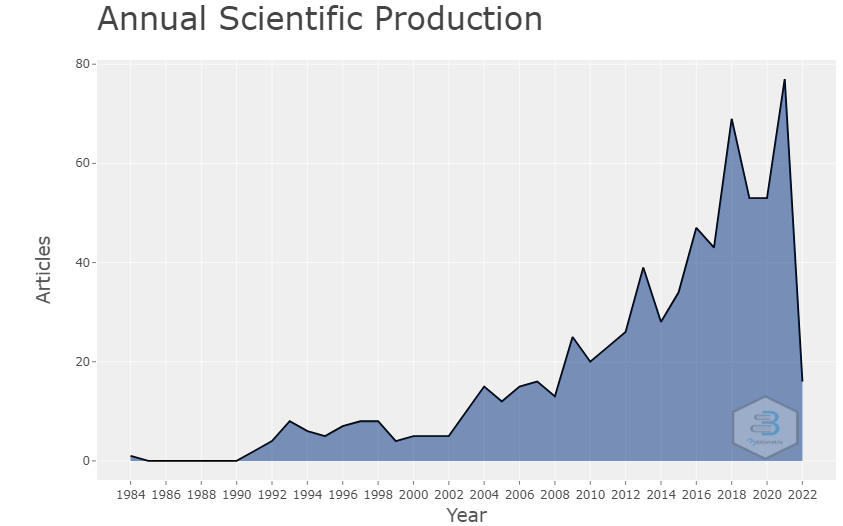
\includegraphics[width=1\textwidth]{experiments/ngsylar/PesqBibliogr/Imagens/ASADES-AnnualScientificProduction.png}
    \caption{Evolução da produção científica no dataset ASADES@ngsylar.}
    \label{fig:evol:anual:ASADES@ngsylar}
\end{figure}

\subsubsection{Interpretação do Crescimento} 

Como visto na figura \ref{fig:evol:anual:ASADES@ngsylar}, a taxa de crescimento do dataset ASADES@ngsylar sugerem que o tema de pesquisa na área de análise e descrição de vídeos tem despertou interesse de forma modesta nos primeiros anos, seguido de um crescimento mais acentuado nos anos seguintes e com tendência de crescimento nos próximos anos. O tema, porém, não parece estar entre as áreas de maior interesse no contexto de produção científica.

\subsection{Evolução das Citações}

A partir do gráfico na figura \ref{fig:evol:anual:citacoes:ASADES@ngsylar}, é visto que não existe muita estabilidade na curva do número de citações, que variava por cerca de 0 a 4 citações por ano e passou a variar de 2 a 6 citações a partir do ano 2000. O pico de quase 30 citações no ano de 1984 provavelmente deve-se a presença de um artigo no dataset publicado neste período e que foi bastante citado.

\begin{figure}[H]
    \centering
    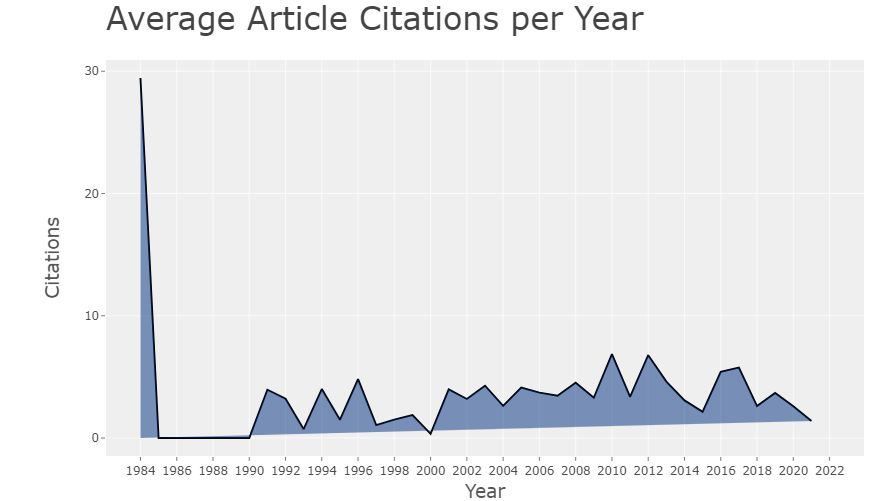
\includegraphics[width=1\textwidth]{experiments/ngsylar/PesqBibliogr/Imagens/ASADES-CitationsYear.png}
    \caption{Evolução das citações no dataset ASADES@ngsylar.}
    \label{fig:evol:anual:citacoes:ASADES@ngsylar}
\end{figure}

\subsubsection{Interpretação das Citações}
Dado o crescimento de produção científica na área, o modesto crescimento na média de citações a cada 20 anos sugere uma tendência de crescimento da bibliografia. Entretanto, deve-se observar com cautela o comportamento da curva nos próximos anos, visto que houveram momentos de queda bruscas na última década.


\subsection{\textit{Plotagem de Três Campos (Diagrama de Sankey)}}
A figura \ref{fig:ASADES@ngsylar:ThreeFieldPlot} apresenta a afinidade entre três diferentes conjuntos de atributos que se correlacionam entre si, sendo estes as 20 citações mais frequentes, os 20 mais proeminentes e as palavras-chaves mais frequentes, da esquerda à direita respectivamente.

\begin{figure}[H]
    \centering
    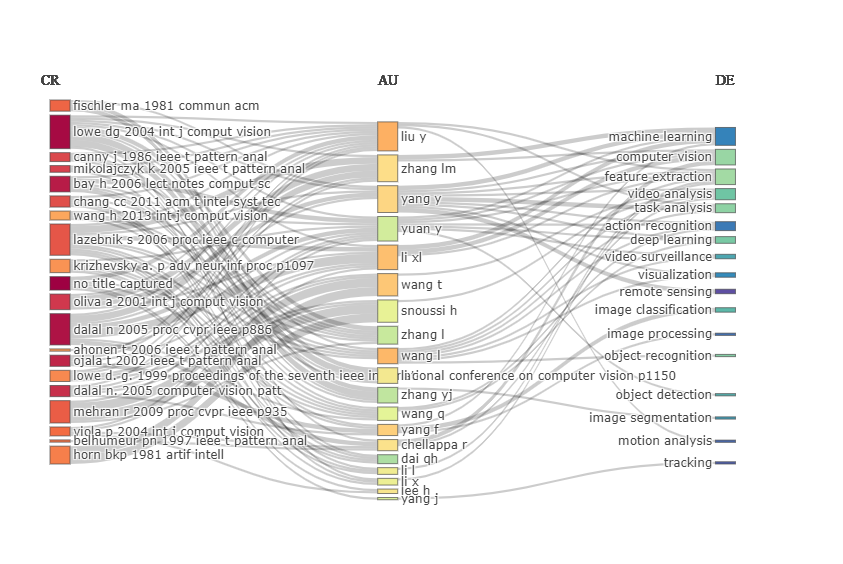
\includegraphics[angle=0,width=1\textwidth]{experiments/ngsylar/PesqBibliogr/Imagens/ASADES-TFPRefAutKeyw.png}
    \caption{Plotagem ``Três Campos'' do dataset ASADES@ngsylar: 20 Autores para Referências e Palavras-Chave mais proeminentes.}
    \label{fig:ASADES@ngsylar:ThreeFieldPlot}
\end{figure}

\subsubsection{Interpretação do diagrama da figura \ref{fig:ASADES@ngsylar:ThreeFieldPlot}}
Os termos mais recorrentes são \textit{machine learning} e \textit{computer vision}, seguidos por termos como \textit{video analysis}, o que sugere a relevância da aplicação de inteligência artificial e apredizado de máquina no processo de análise de vídeo e classificação de imagens.
Aguns outros termos como \textit{object recognition} aparecem em menor escala, indicando a aplicação de estudos baseados no tema para analise de imagens capturadas em tempo real por robôs.
O lado esquerdo do diagram sugere alguns dos artigos mais relevantes para embasamento de estudos relacionados ao tema de análise e descrição de vídeos.

\subsection{Análises Bibliométricas}

\begin{figure}[H]
    \centering
    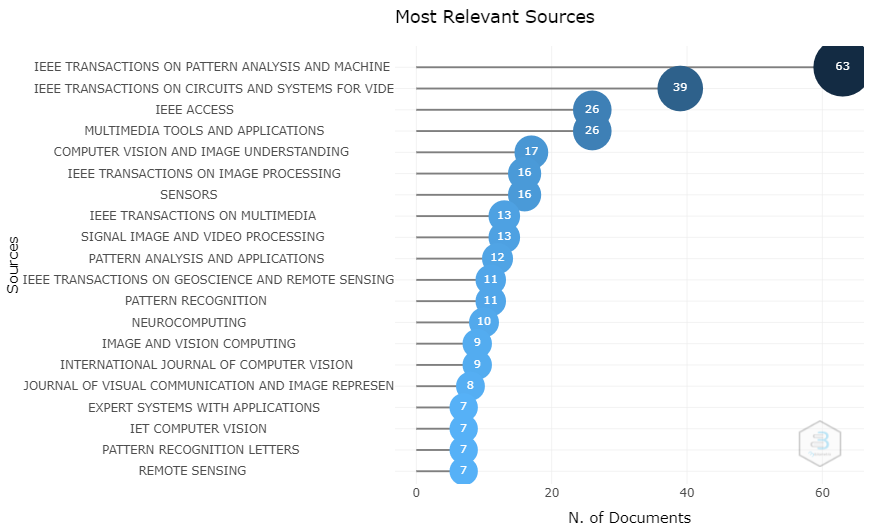
\includegraphics[angle=0,width=1\textwidth]{experiments/ngsylar/PesqBibliogr/Imagens/ASADES-MostRelevantSources.png}
    \caption{Fontes de Informação mais Relevantes no dataset ASADES@ngsylar.}
    \label{fig:ASADES@ngsylar:RelevantSources}
\end{figure}

\begin{figure}[H]
    \centering
    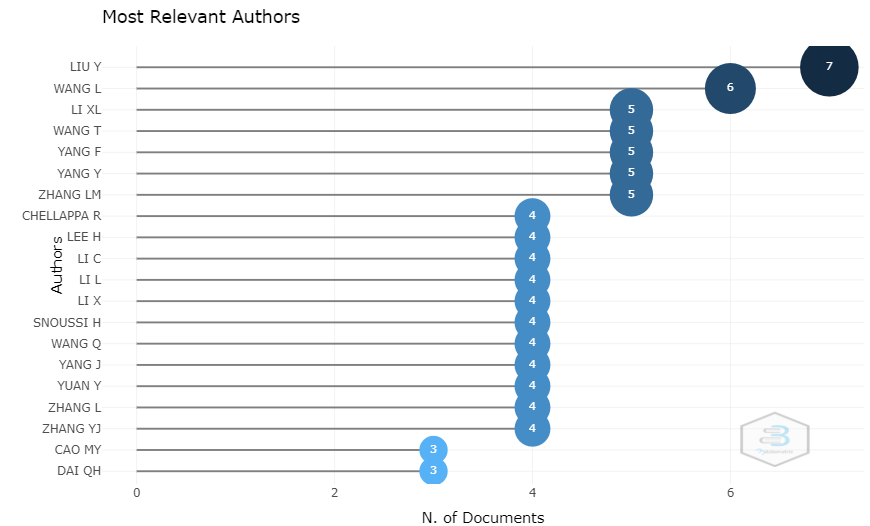
\includegraphics[angle=0,width=1\textwidth]{experiments/ngsylar/PesqBibliogr/Imagens/ASADES-MostRelevantAuthors.png}
    \caption{Nomes de autores com maior relevância no dataset ASADES@ngsylar.}
    \label{fig:ASADES@ngsylar:RelevantAuthors}
\end{figure}

\begin{figure}[H]
    \centering
    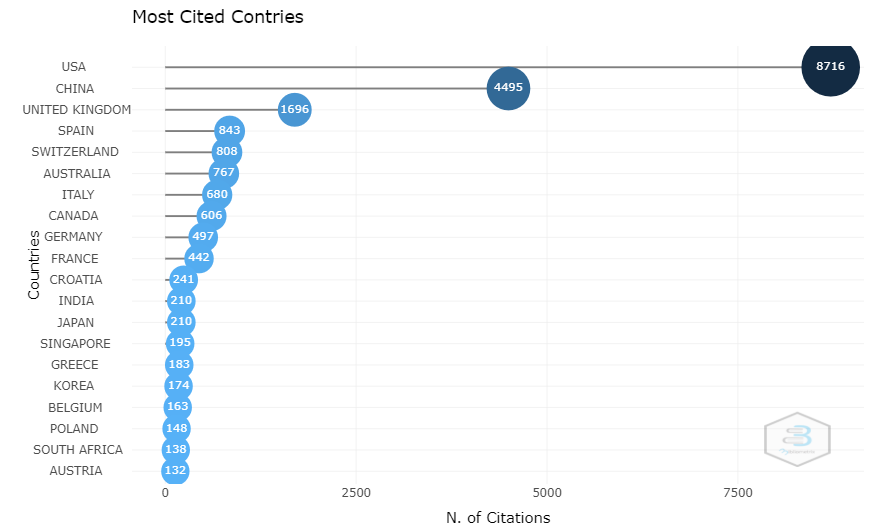
\includegraphics[angle=0,width=1\textwidth]{experiments/ngsylar/PesqBibliogr/Imagens/ASADES-MostCitedCountries.png}
    \caption{Países mais citados no dataset ASADES@ngsylar.}
    \label{fig:ASADES@ngsylar:MostCitedCountries}
\end{figure}

\subsubsection{Interpretação das figuras }

A figura \ref{fig:ASADES@ngsylar:RelevantSources} mostra as principais fontes de informação onde se encontram os artigos presentes no dataset ASADE@ngylar, destacando as \textit{IEEE Transactions on Pattern Analysis and Machine} e \textit{IEEE Transactions on Circuits and Systems for Vide}.
Na figura \ref{fig:ASADES@ngsylar:MostCitedCountries}, entre os países mais citados, é visto que maior parte da produção encontra-se nos Estados Unidos, seguido pela China e logo após pelo Reino Unido.



















\subsection{Análises Bibliométricas: Autores}

Para a análise acerca dos Autores, devemos considerar as seguintes imagens abaixo.

\begin{figure}[H]
    \centering
    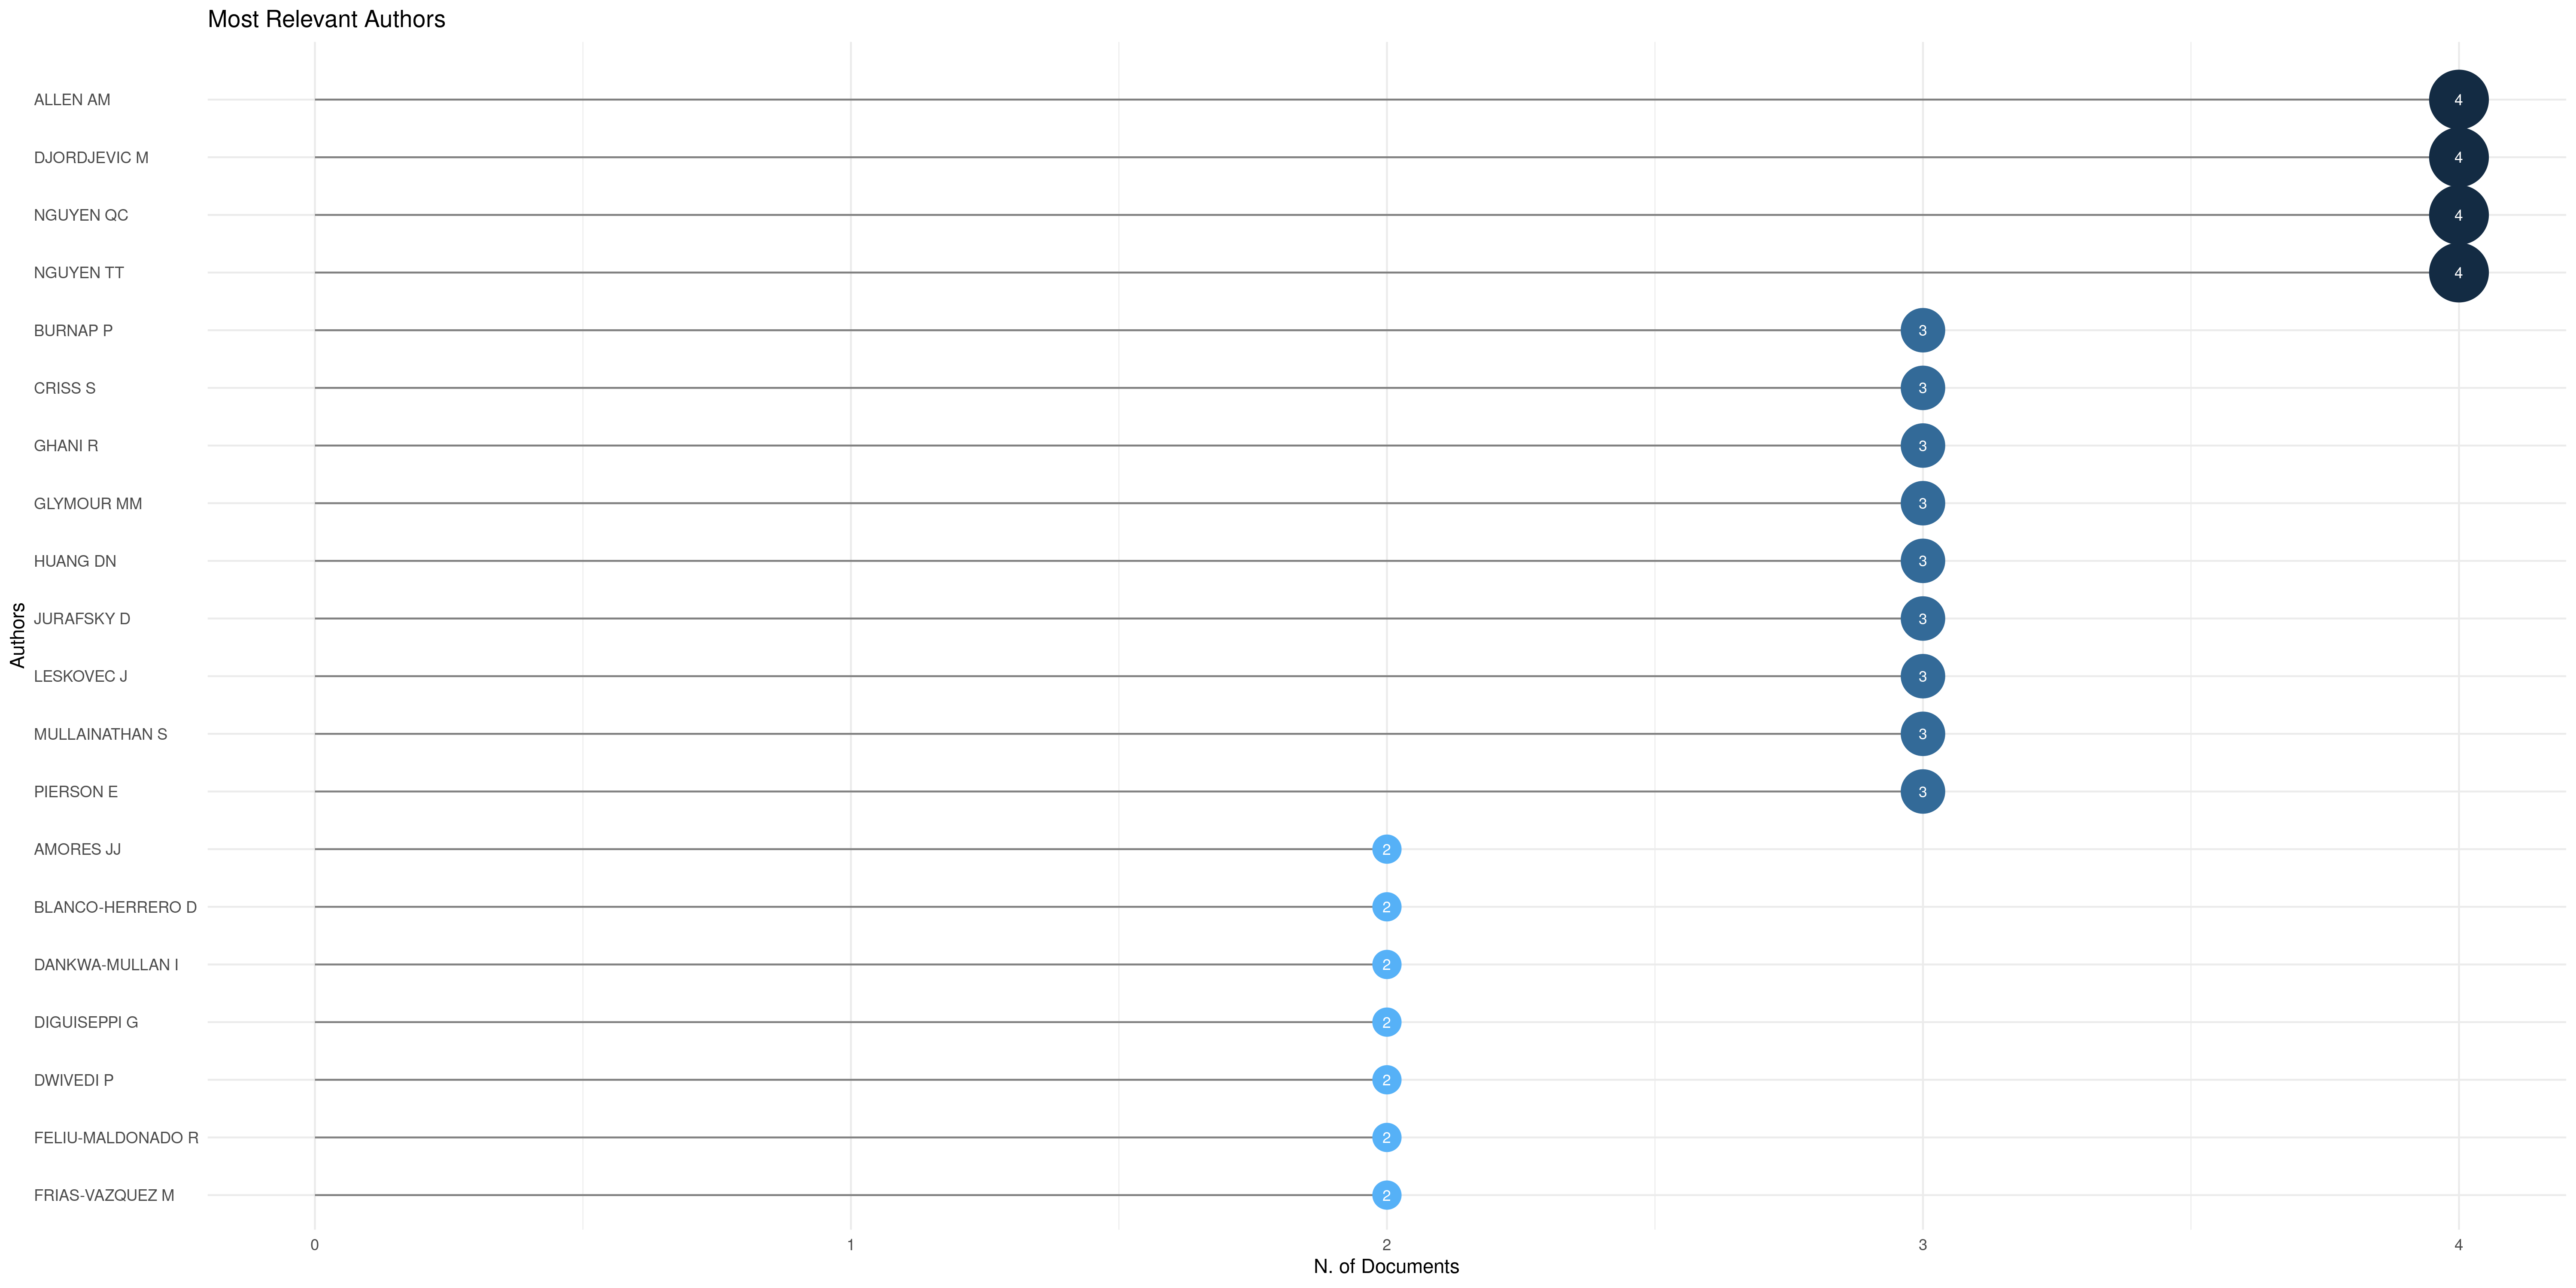
\includegraphics[angle=0,width=1\textwidth]{experiments/ngsylar/PesqBibliogr/Imagens/MostRelevantAuthors-2022-02-09.png}
    \caption{Autores relevantes do dataset ASADES@ngsylar.}
    \label{fig:ASADES@ngsylar:RelevantAuthors}
\end{figure}

\begin{figure}[H]
    \centering
    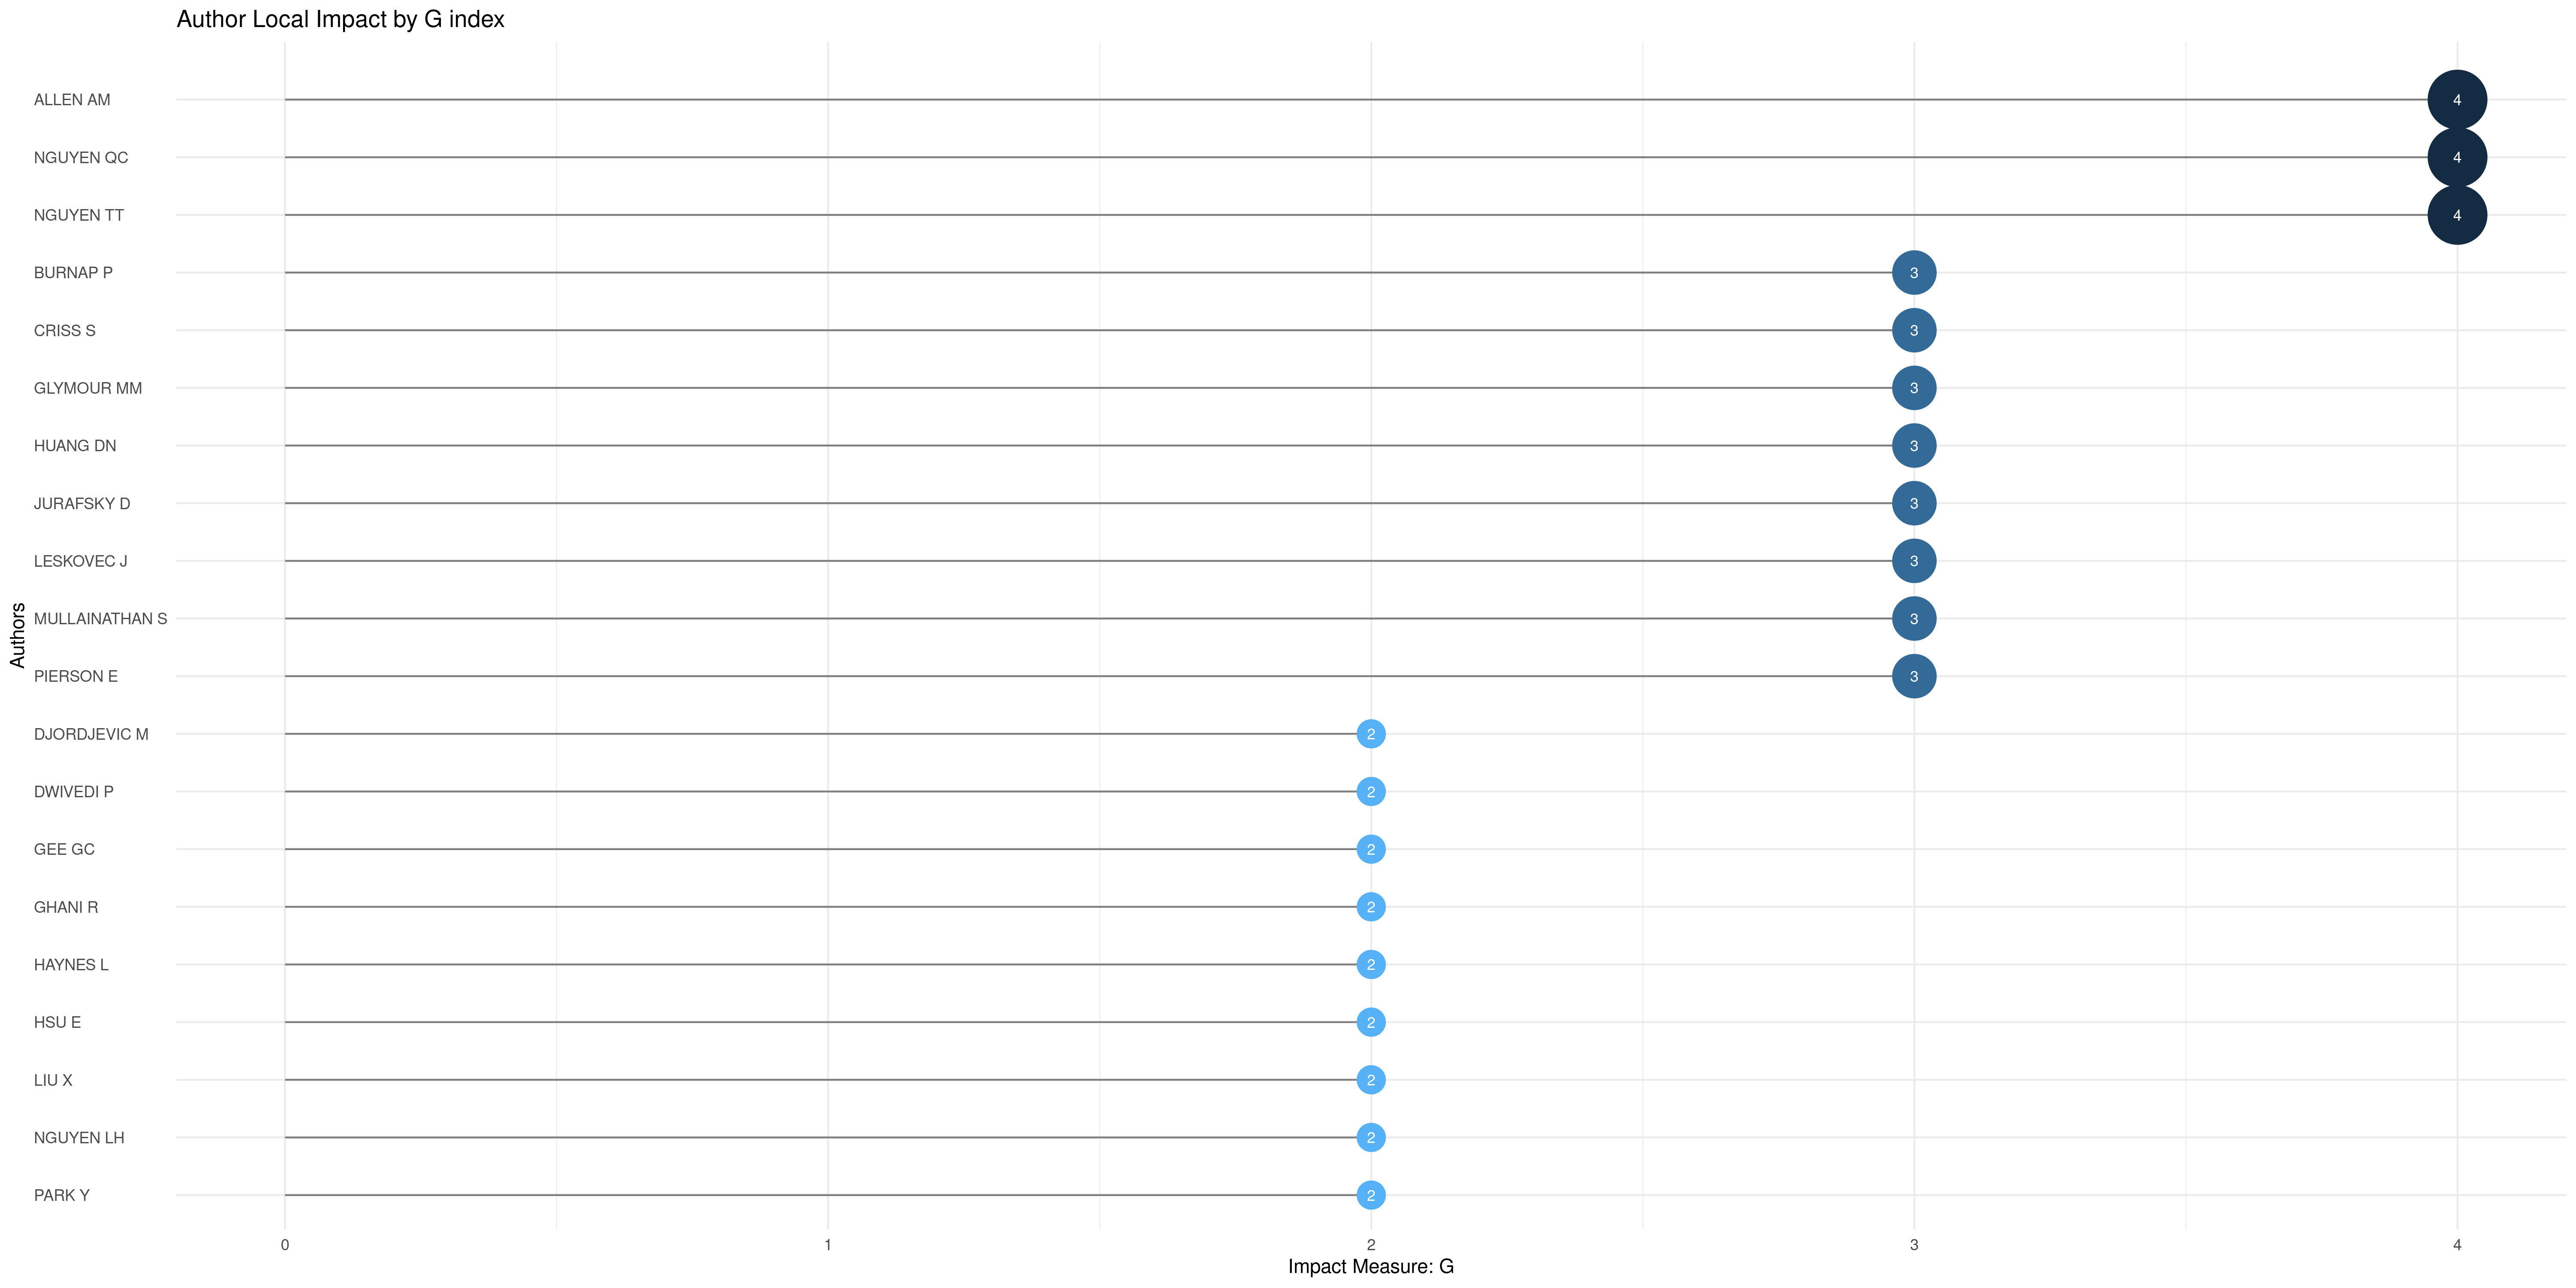
\includegraphics[angle=0,width=1\textwidth]{experiments/ngsylar/PesqBibliogr/Imagens/AuthorImpact-2022-02-09.png}
    \caption{Impacto dos Autores no dataset ASADES@ngsylar.}
    \label{fig:ASADES@ngsylar:AuthorsImpact}
\end{figure}

\begin{figure}[H]
    \centering
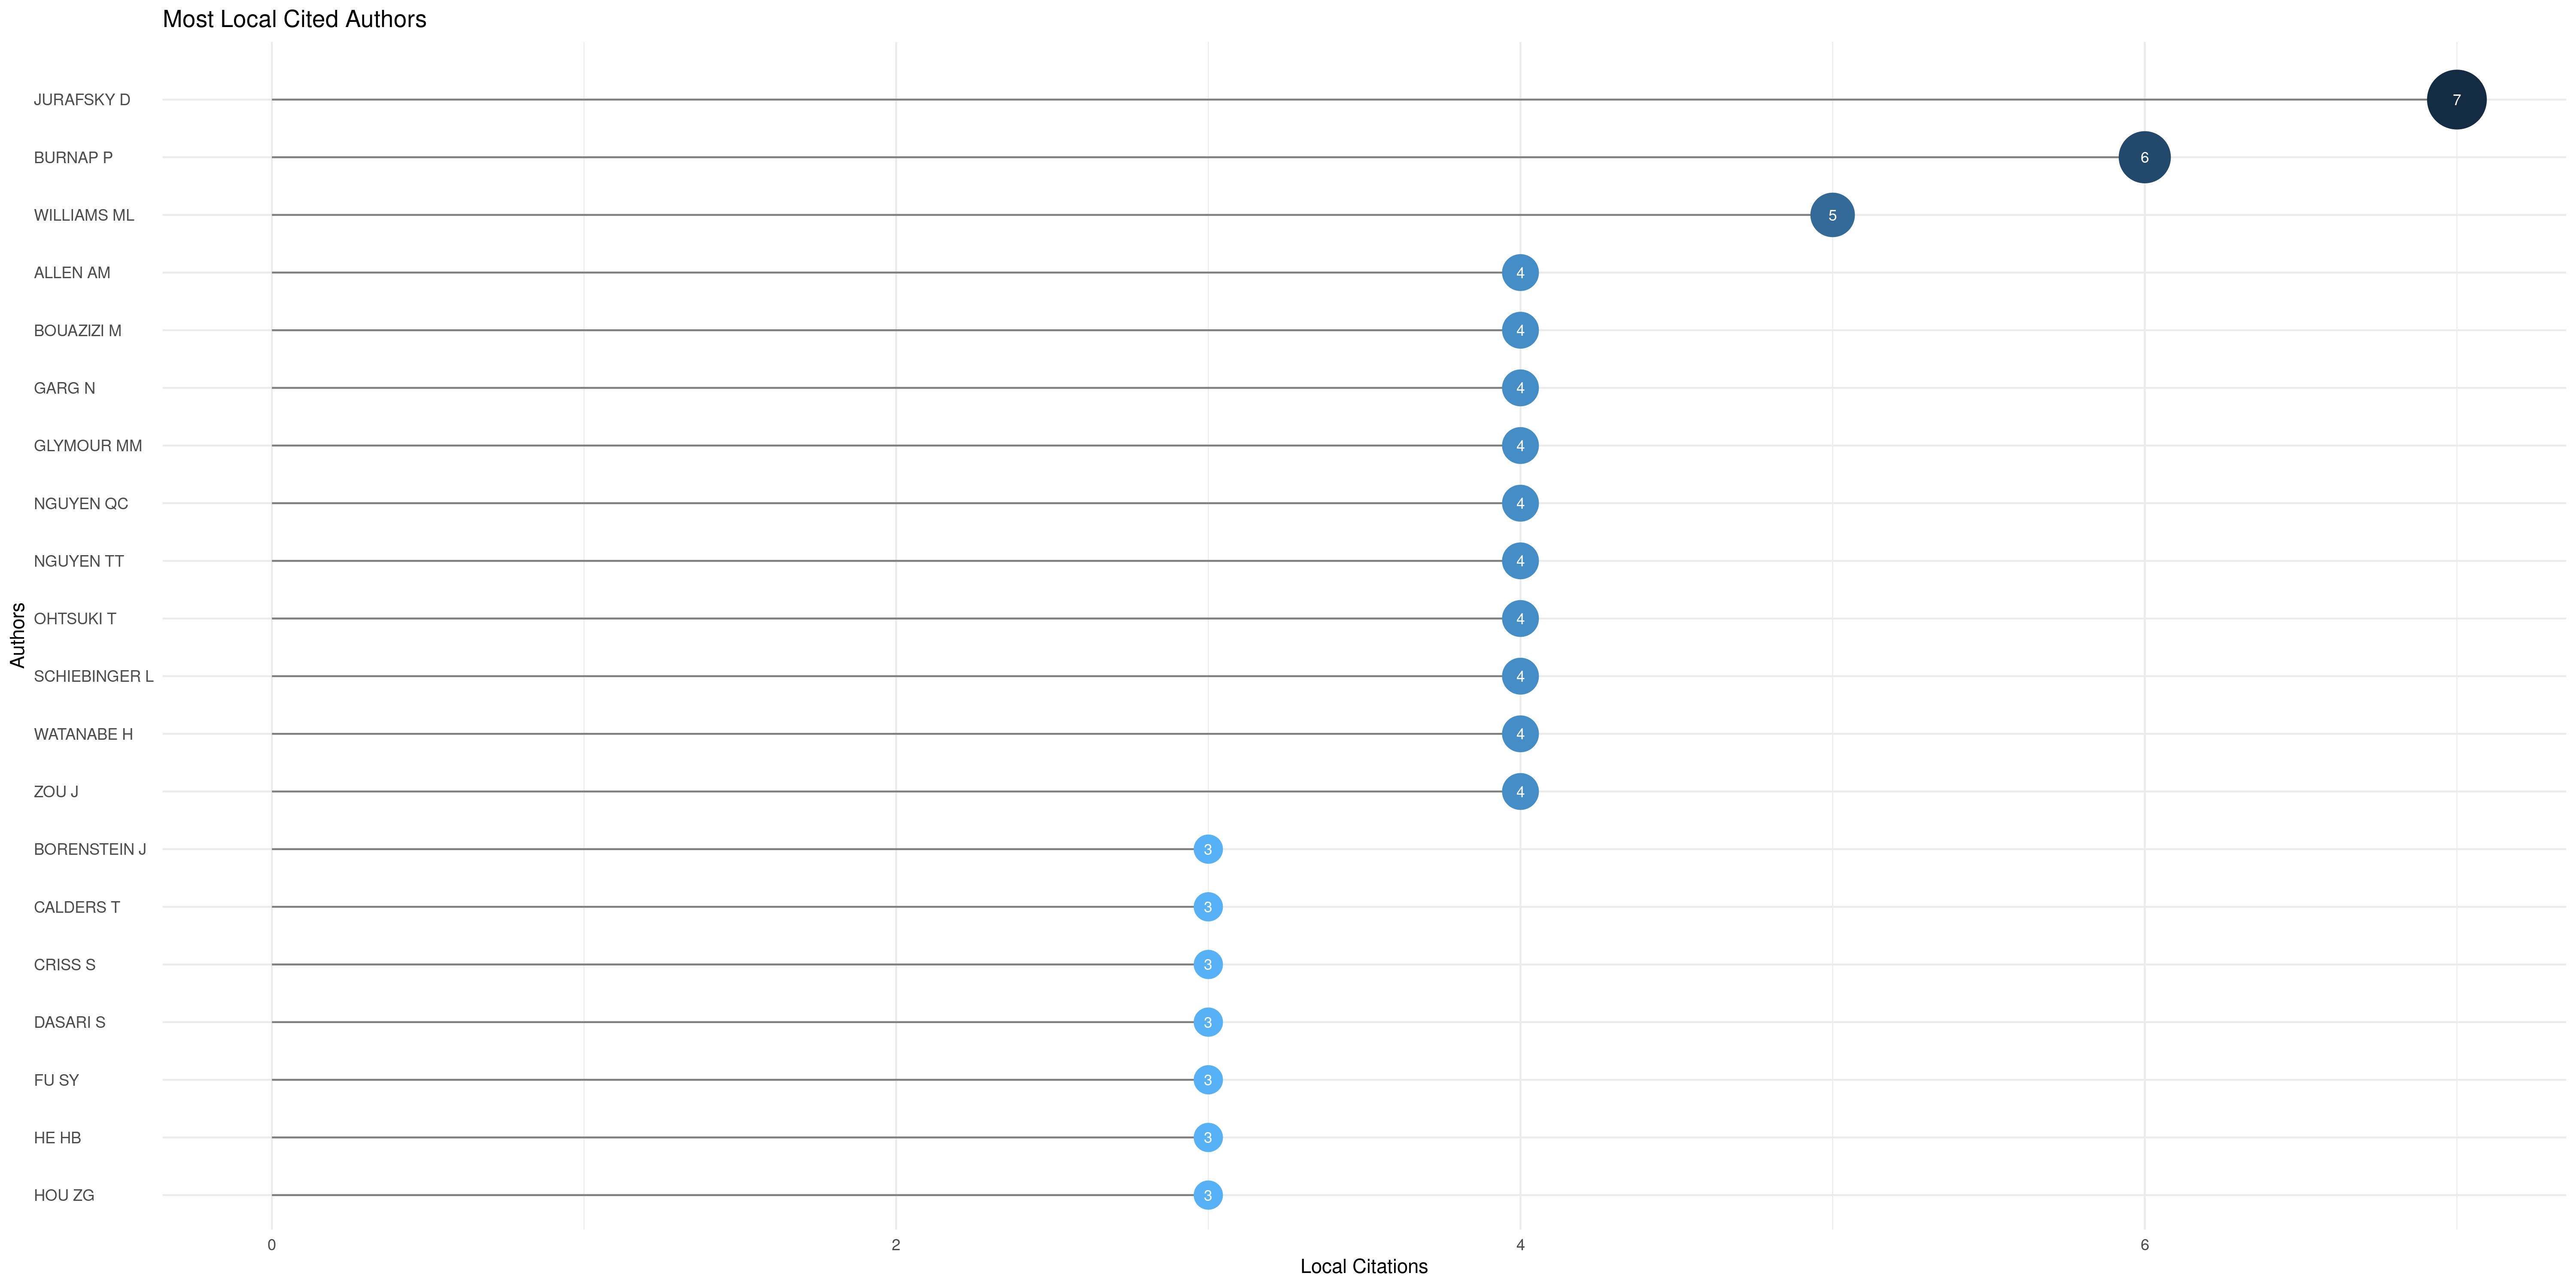
\includegraphics[angle=0,width=1\textwidth]{experiments/ngsylar/PesqBibliogr/Imagens/MostLocalCitedAuthors-2022-02-09.png}
    \caption{Autores locais mais citados do dataset ASADES@ngsylar.}
    \label{fig:ASADES@ngsylar:MostCitedAuthors}
\end{figure}

\begin{figure}[H]
    \centering
    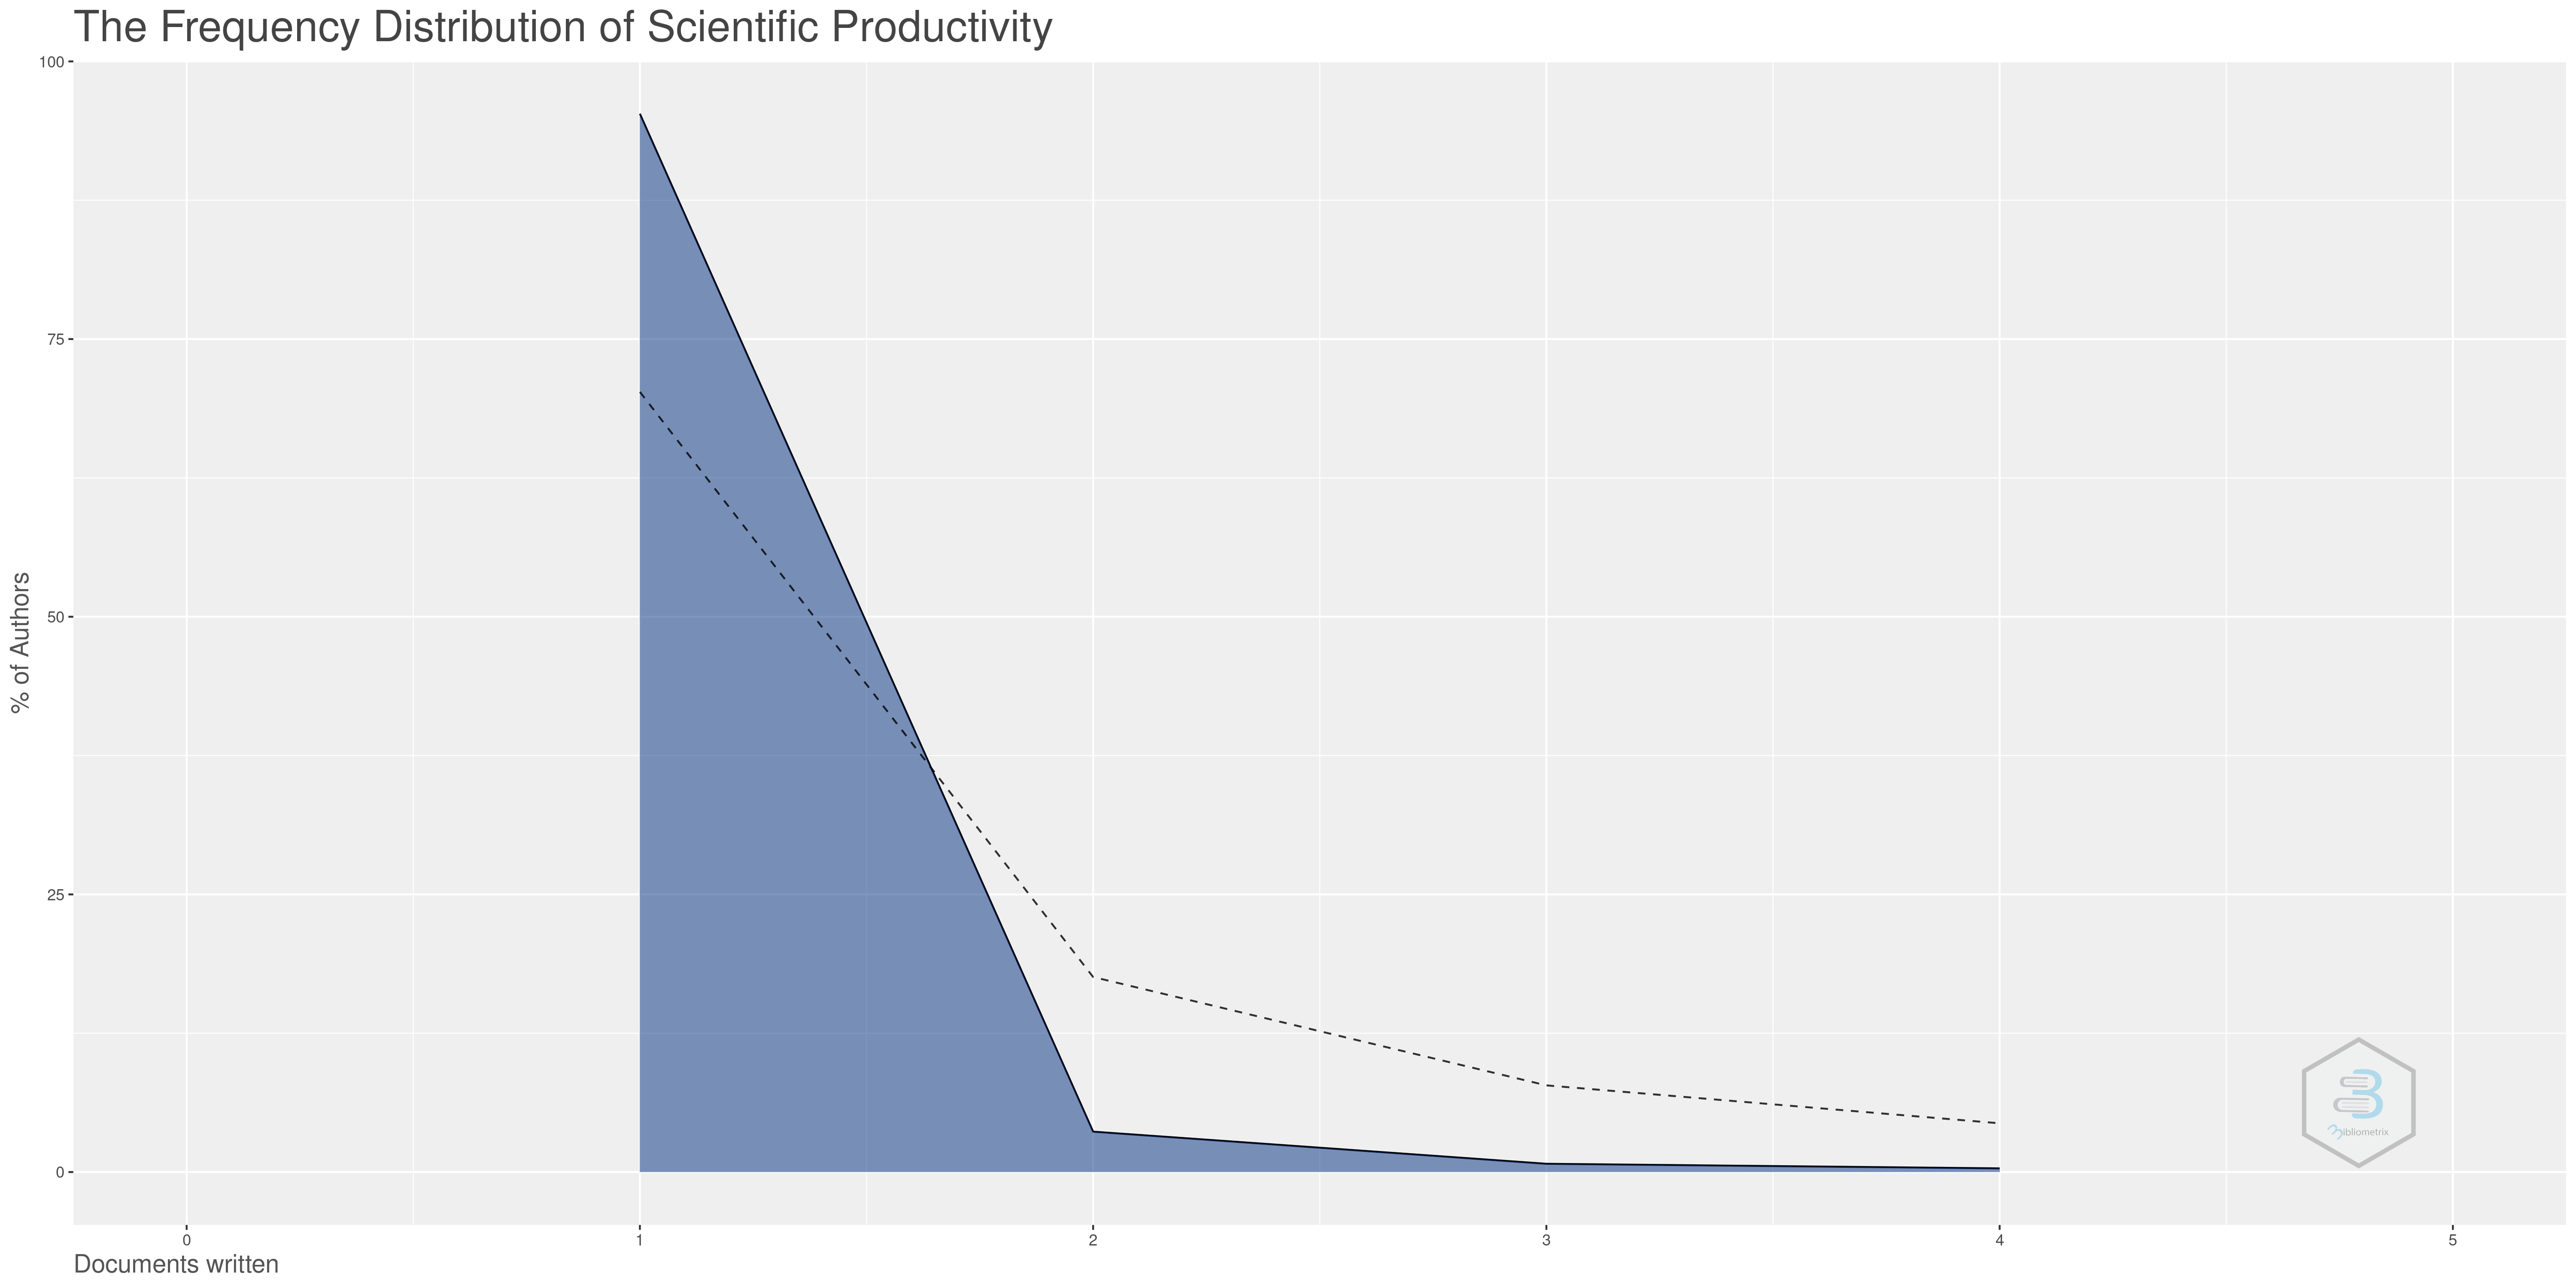
\includegraphics[angle=0,width=1\textwidth]{experiments/ngsylar/PesqBibliogr/Imagens/LotkaLaw-2022-02-09.png}
    \caption{Frequência de publição dos artigos dos Autores do dataset ASADES@ngsylar. (Lei de Lotka)}
    \label{fig:ASADES@ngsylar:Lotka}
\end{figure}

\subsubsection{Interpretação das figuras }
As figuras \ref{fig:ASADES@ngsylar:RelevantAuthors}, \ref{fig:ASADES@ngsylar:AuthorsImpact} e \ref{fig:ASADES@ngsylar:MostCitedAuthors} nos auxiliam a identificar os autores mais relevantes, os que mais influenciam e quais são os mais citado dentro do própio conjunto de dados.

Entretanto, considerando a figura \ref{fig:ASADES@ngsylar:Lotka} podemos ver que quase 100\% dos autores possuem apenas um artigo referente ao tema, consequentemente, não há continuação da pesquisa nessa área --- basta ver a drástica queda na porcentagem de autores que possuem um para dois artigos. Desse modo, tomando em consideração a curva pontilhada, vemos que as publicações referentes ao assunto estão consideravelmente fora do padrão esperado. Tendo isso em vista, há uma perda na qualidade da produção científica pois não ocorre o aprofundamento nesse campo o que dificulta o desenvolvimento de bons artigos de referência.


\subsection{Análises Bibliométricas: Documentos}

Para enriquecer a compreensão da análise acerca dos documentos, primeiro devemos identificar quais são os artigos mais citados globalmente --- não necessariamente estão presentes nesse conjunto de dados -- quais são artigos mais citados dentro do próprio dataset. Portanto, as figuras \ref{fig:ASADES@ngsylar:GlobalCitedDocs} e \ref{fig:ASADES@ngsylar:LocalCitedDocs}, abaixo, nos ajudam a verificar esses parâmetros.

\begin{figure}[H]
    \centering
    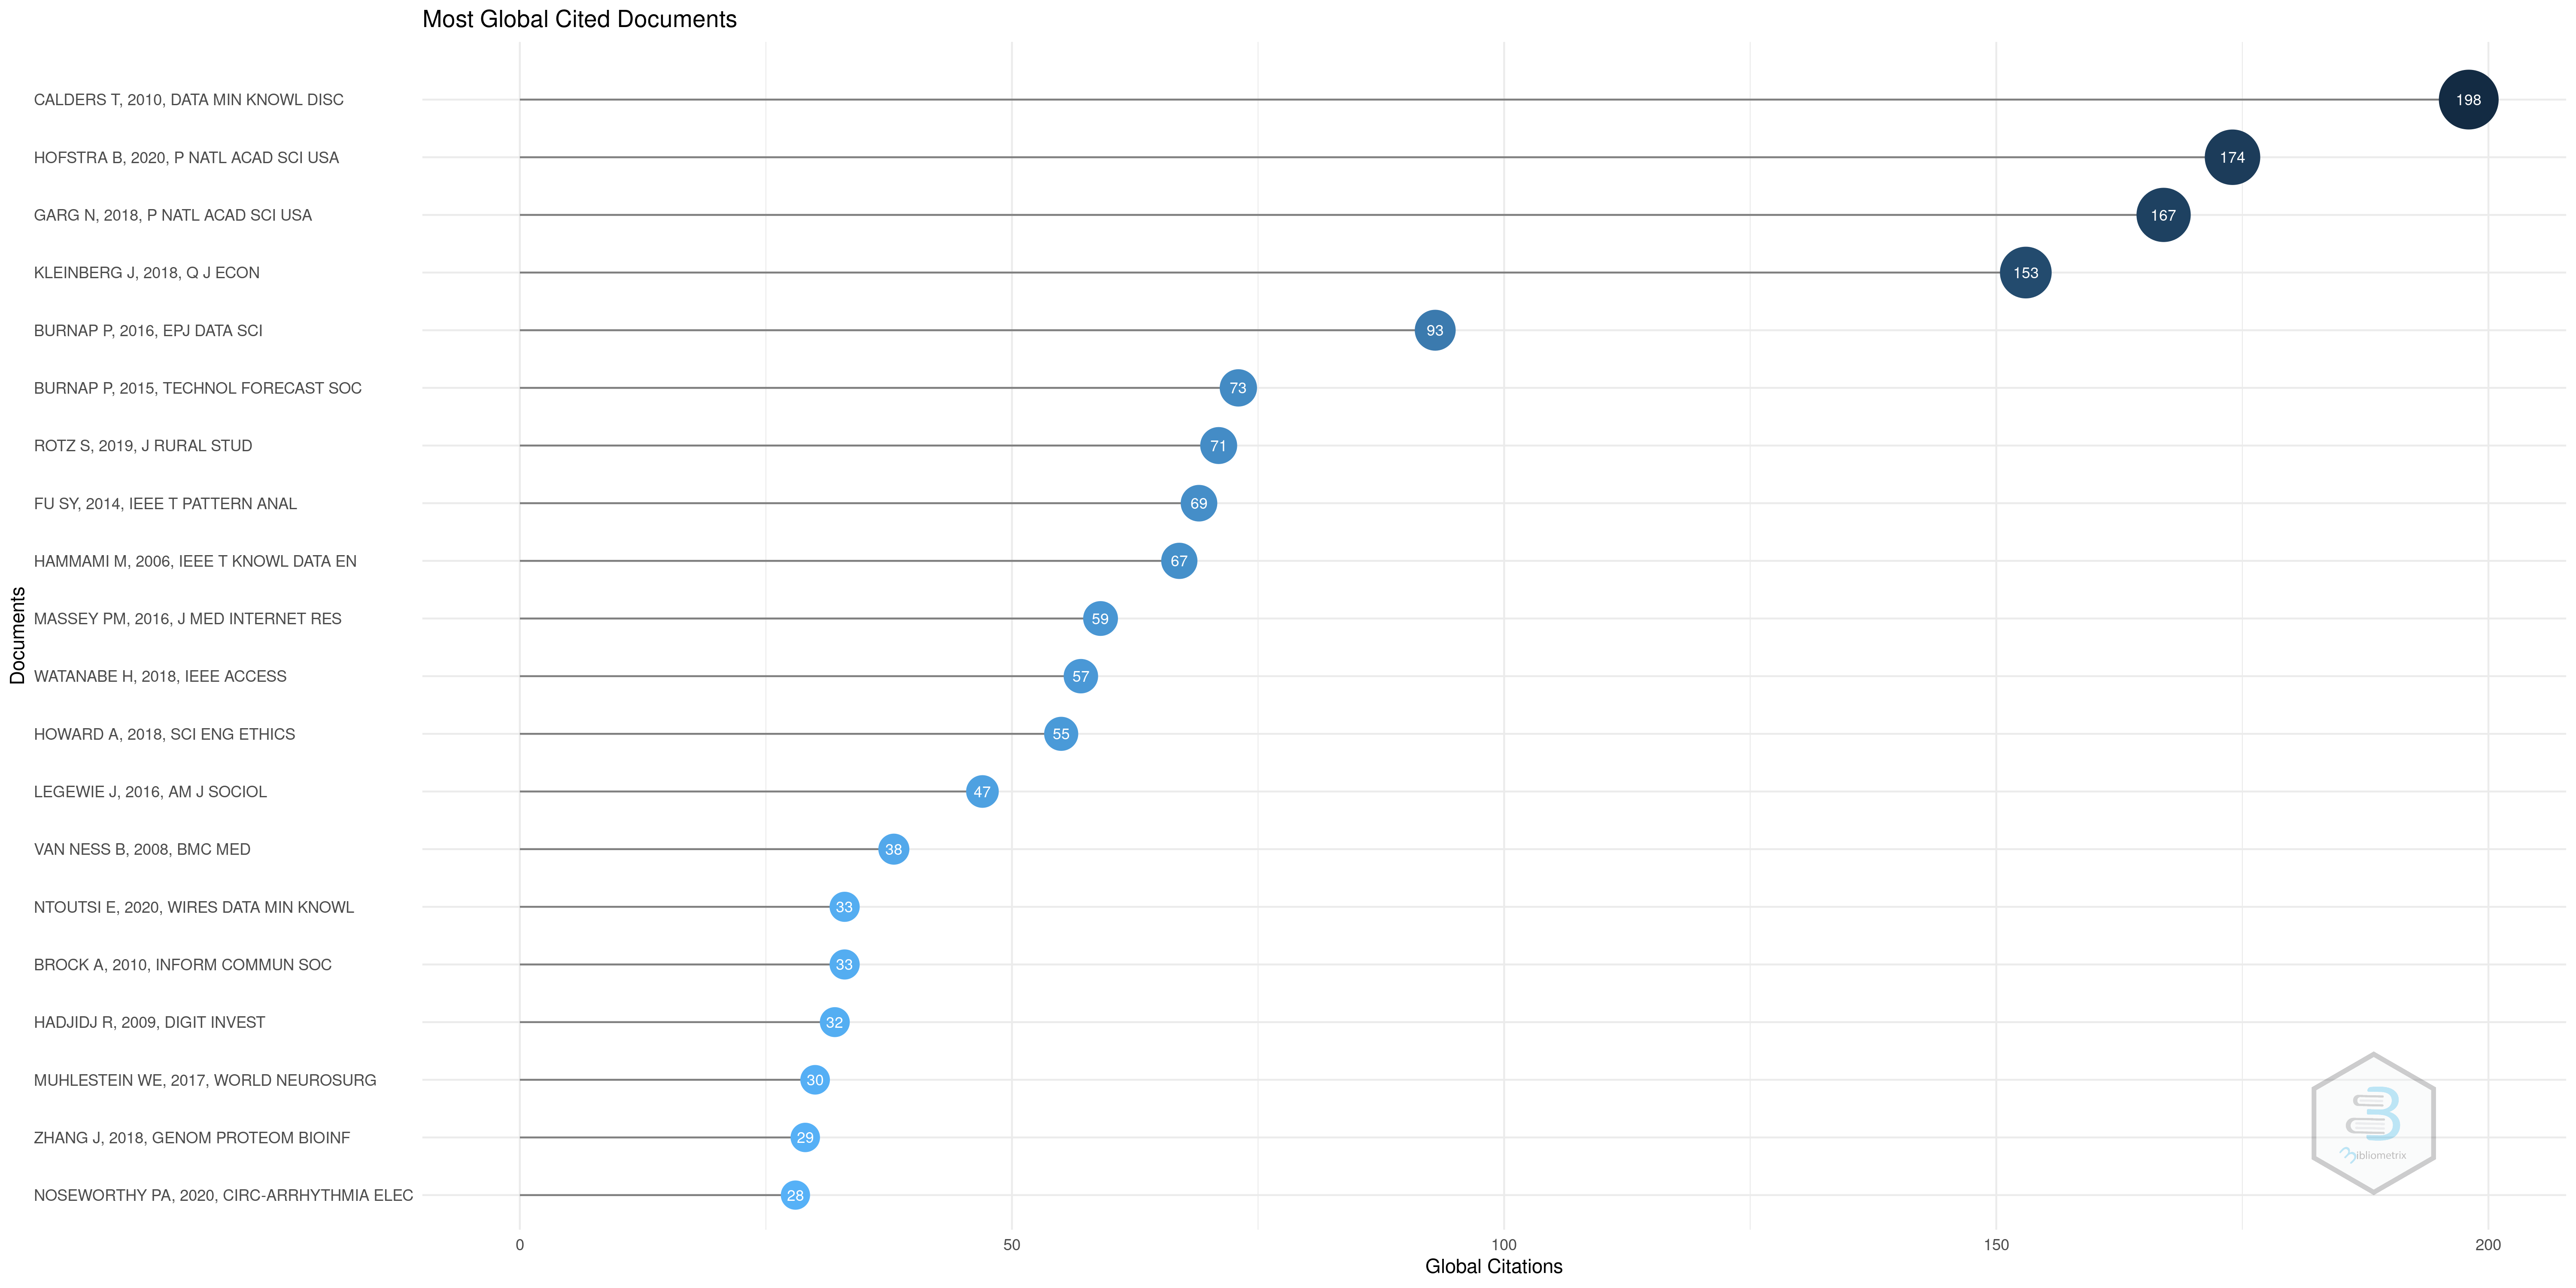
\includegraphics[angle=0,width=1\textwidth]{experiments/ngsylar/PesqBibliogr/Imagens/MostGlobalCitedDocuments-2022-02-09.png}
    \caption{Os artigos globais mais citados do ASADES@ngsylar.}
    \label{fig:ASADES@ngsylar:GlobalCitedDocs}
\end{figure}

\begin{figure}[H]
    \centering
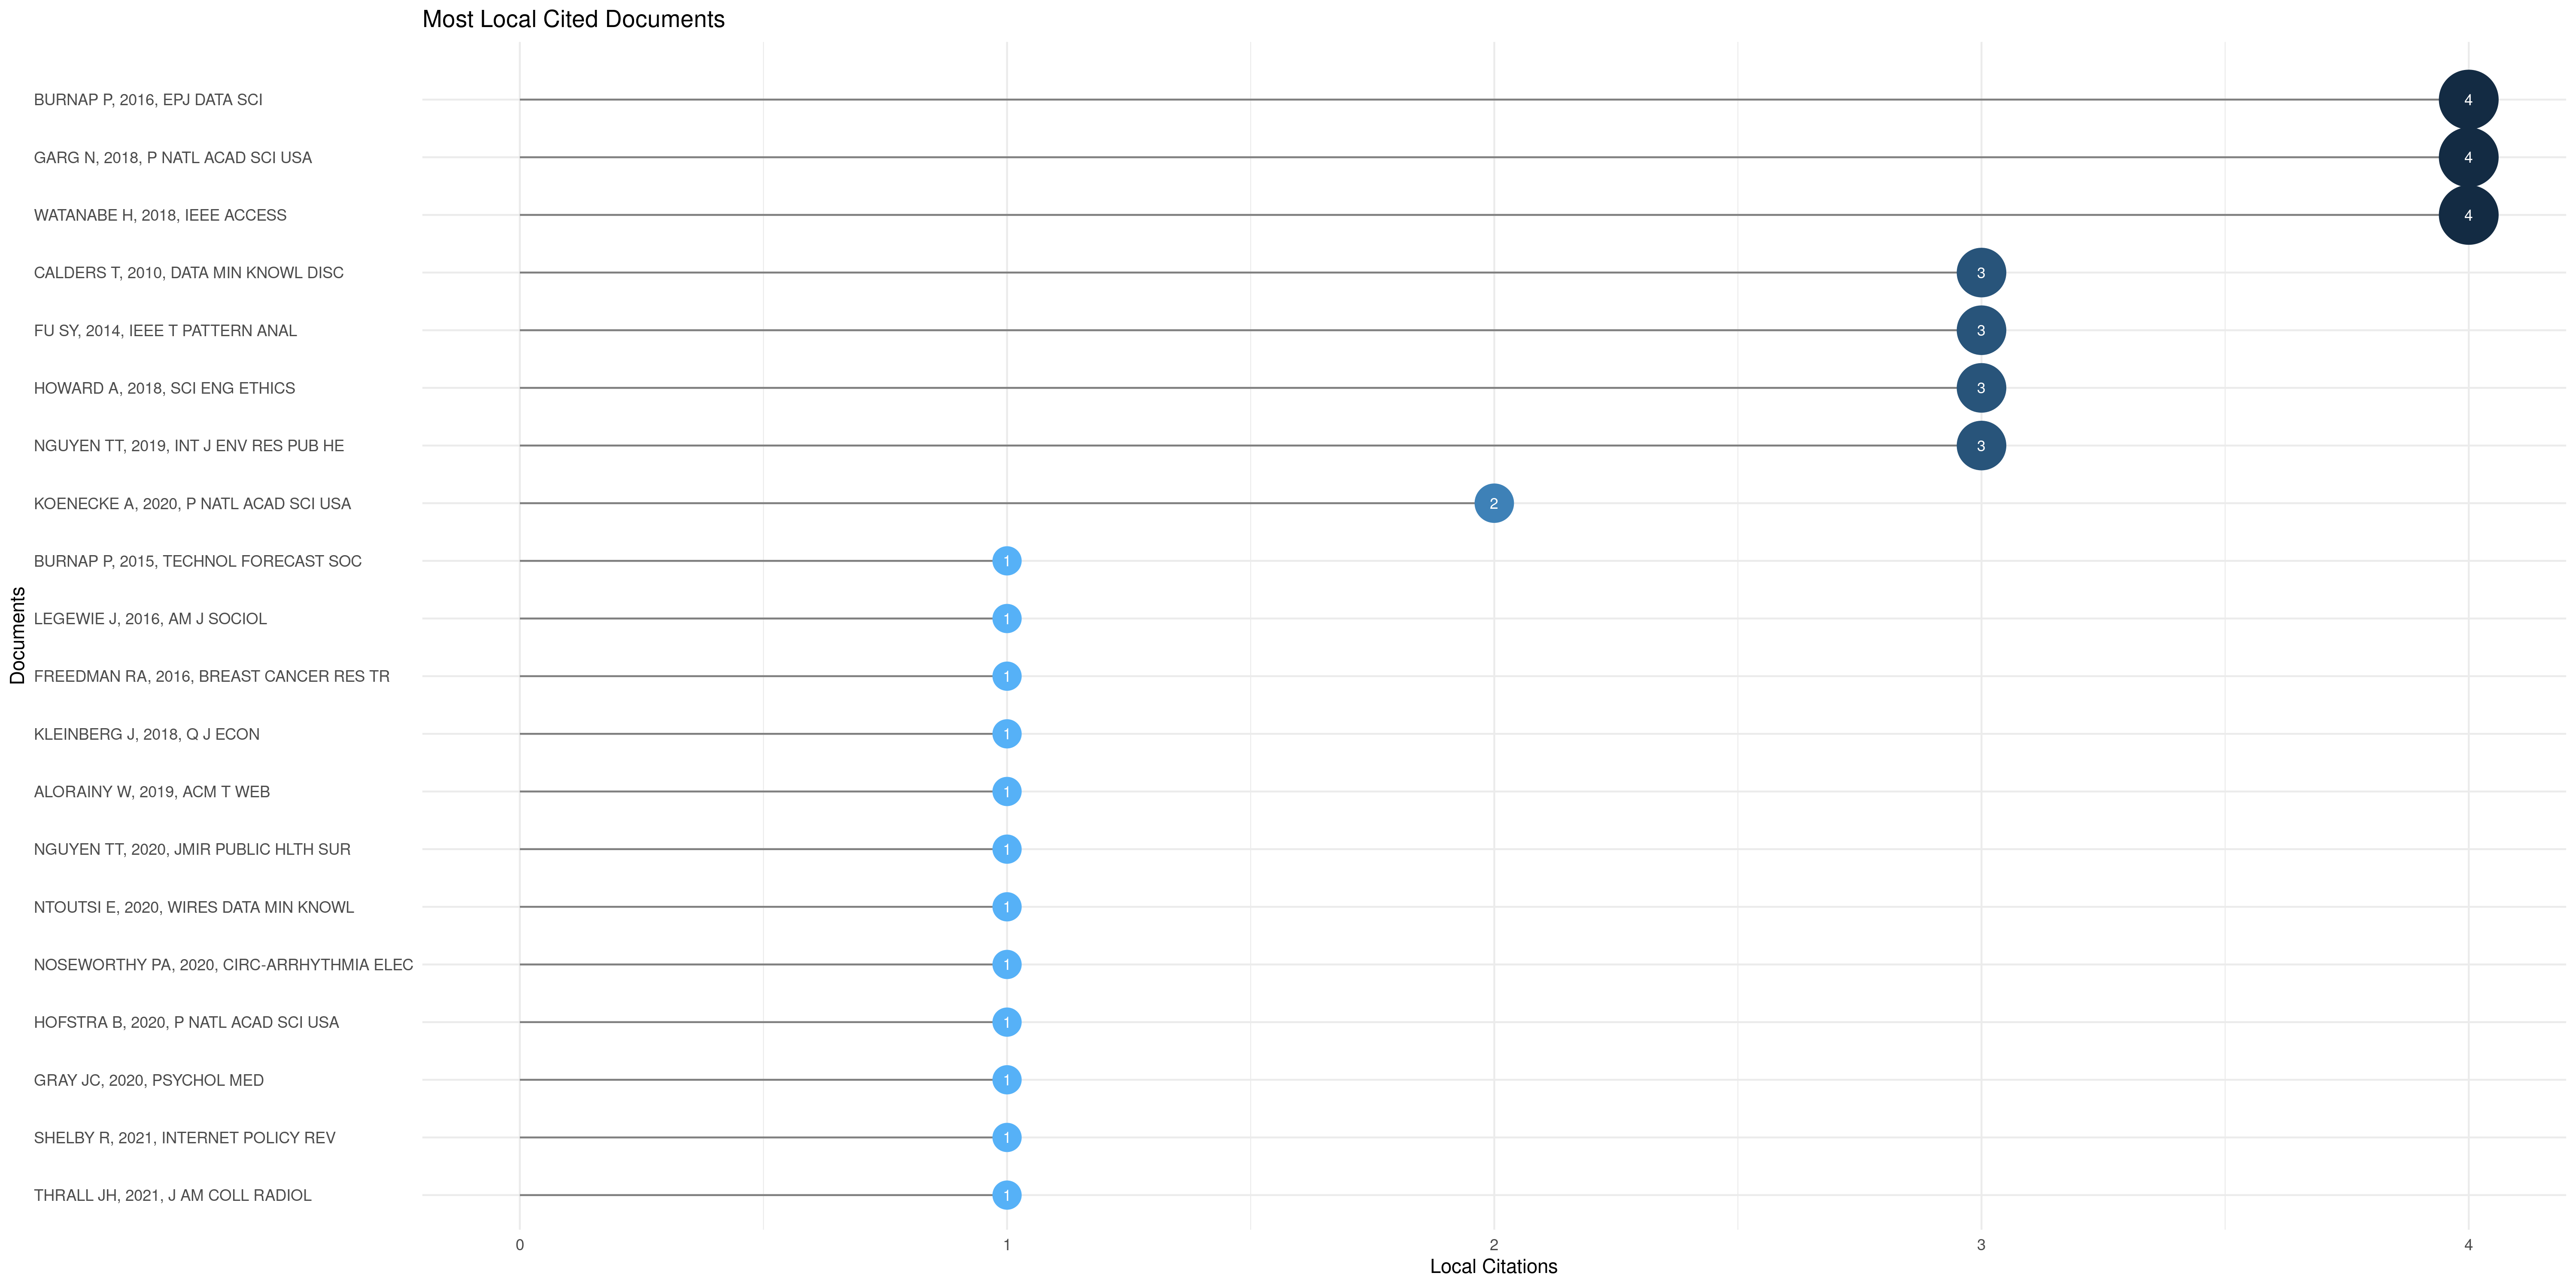
\includegraphics[angle=0,width=1\textwidth]{experiments/ngsylar/PesqBibliogr/Imagens/MostLocalCitedDocuments-2022-02-09.png}
    \caption{Os artigos locais mais citados do ASADES@ngsylar.}
    \label{fig:ASADES@ngsylar:LocalCitedDocs}
\end{figure}

Na secção \ref{sec:ASADES@ngsylar:Citations} foi visto que houve um pico de citações em 2010, podemos ver aqui que o artigo em questão é o \textit{``CALDERS T, 2010, DATA MIN KNOWL DISC''}. Ele aparece tanto na figura \ref{fig:ASADES@ngsylar:GlobalCitedDocs} quanto na \ref{fig:ASADES@ngsylar:LocalCitedDocs}, ao encontrá-lo na base de dados, vemos que seu título é \textit{Three naive Bayes approaches for discrimination-free classification} --- Três abordagens de Naive Bayes para classificação livre de discriminação --- portanto, é possível ver que esse artigo é um dos precursores do debate que estamos enfocando, o iniciando no início da década passada, em 2010.

\begin{figure}[H]
    \centering
    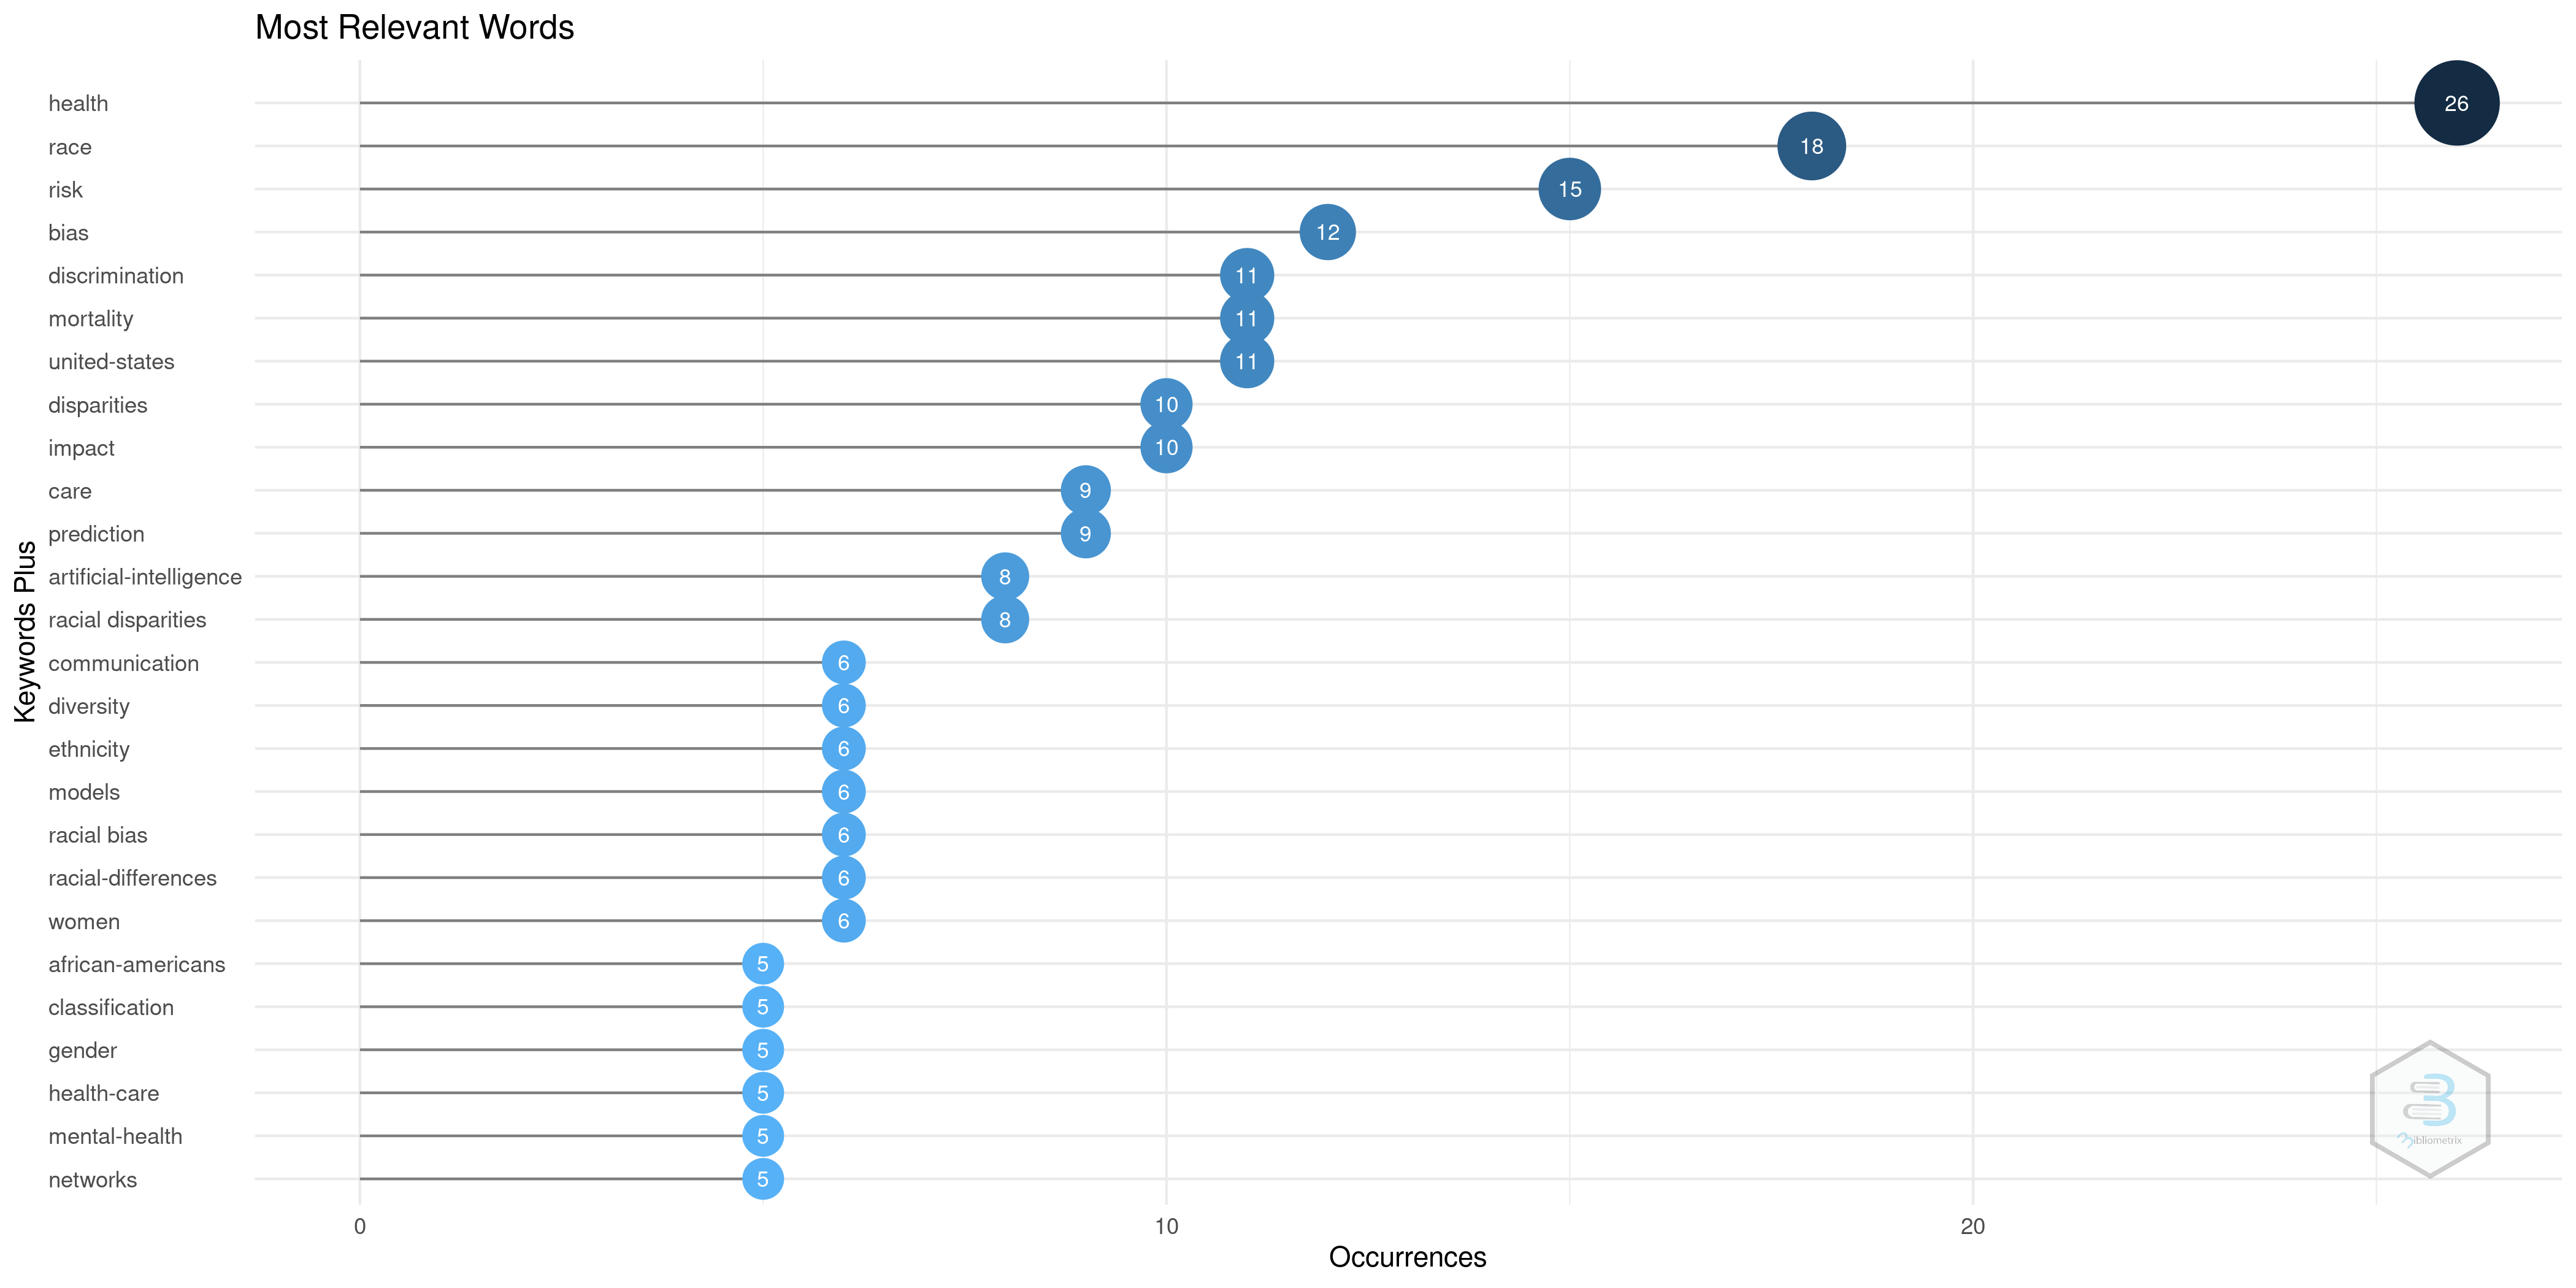
\includegraphics[angle=0,width=1\textwidth]{experiments/ngsylar/PesqBibliogr/Imagens/MostRelevantWords-2022-02-09.png}
    \caption{As 20 palavras mais relevantes dentro do dataset ASADES@ngsylar --- utilizando como parâmetro as Keywords Plus}
    \label{fig:ASADES@ngsylar:RelevantWords}
\end{figure}

\begin{figure}[H]
    \centering
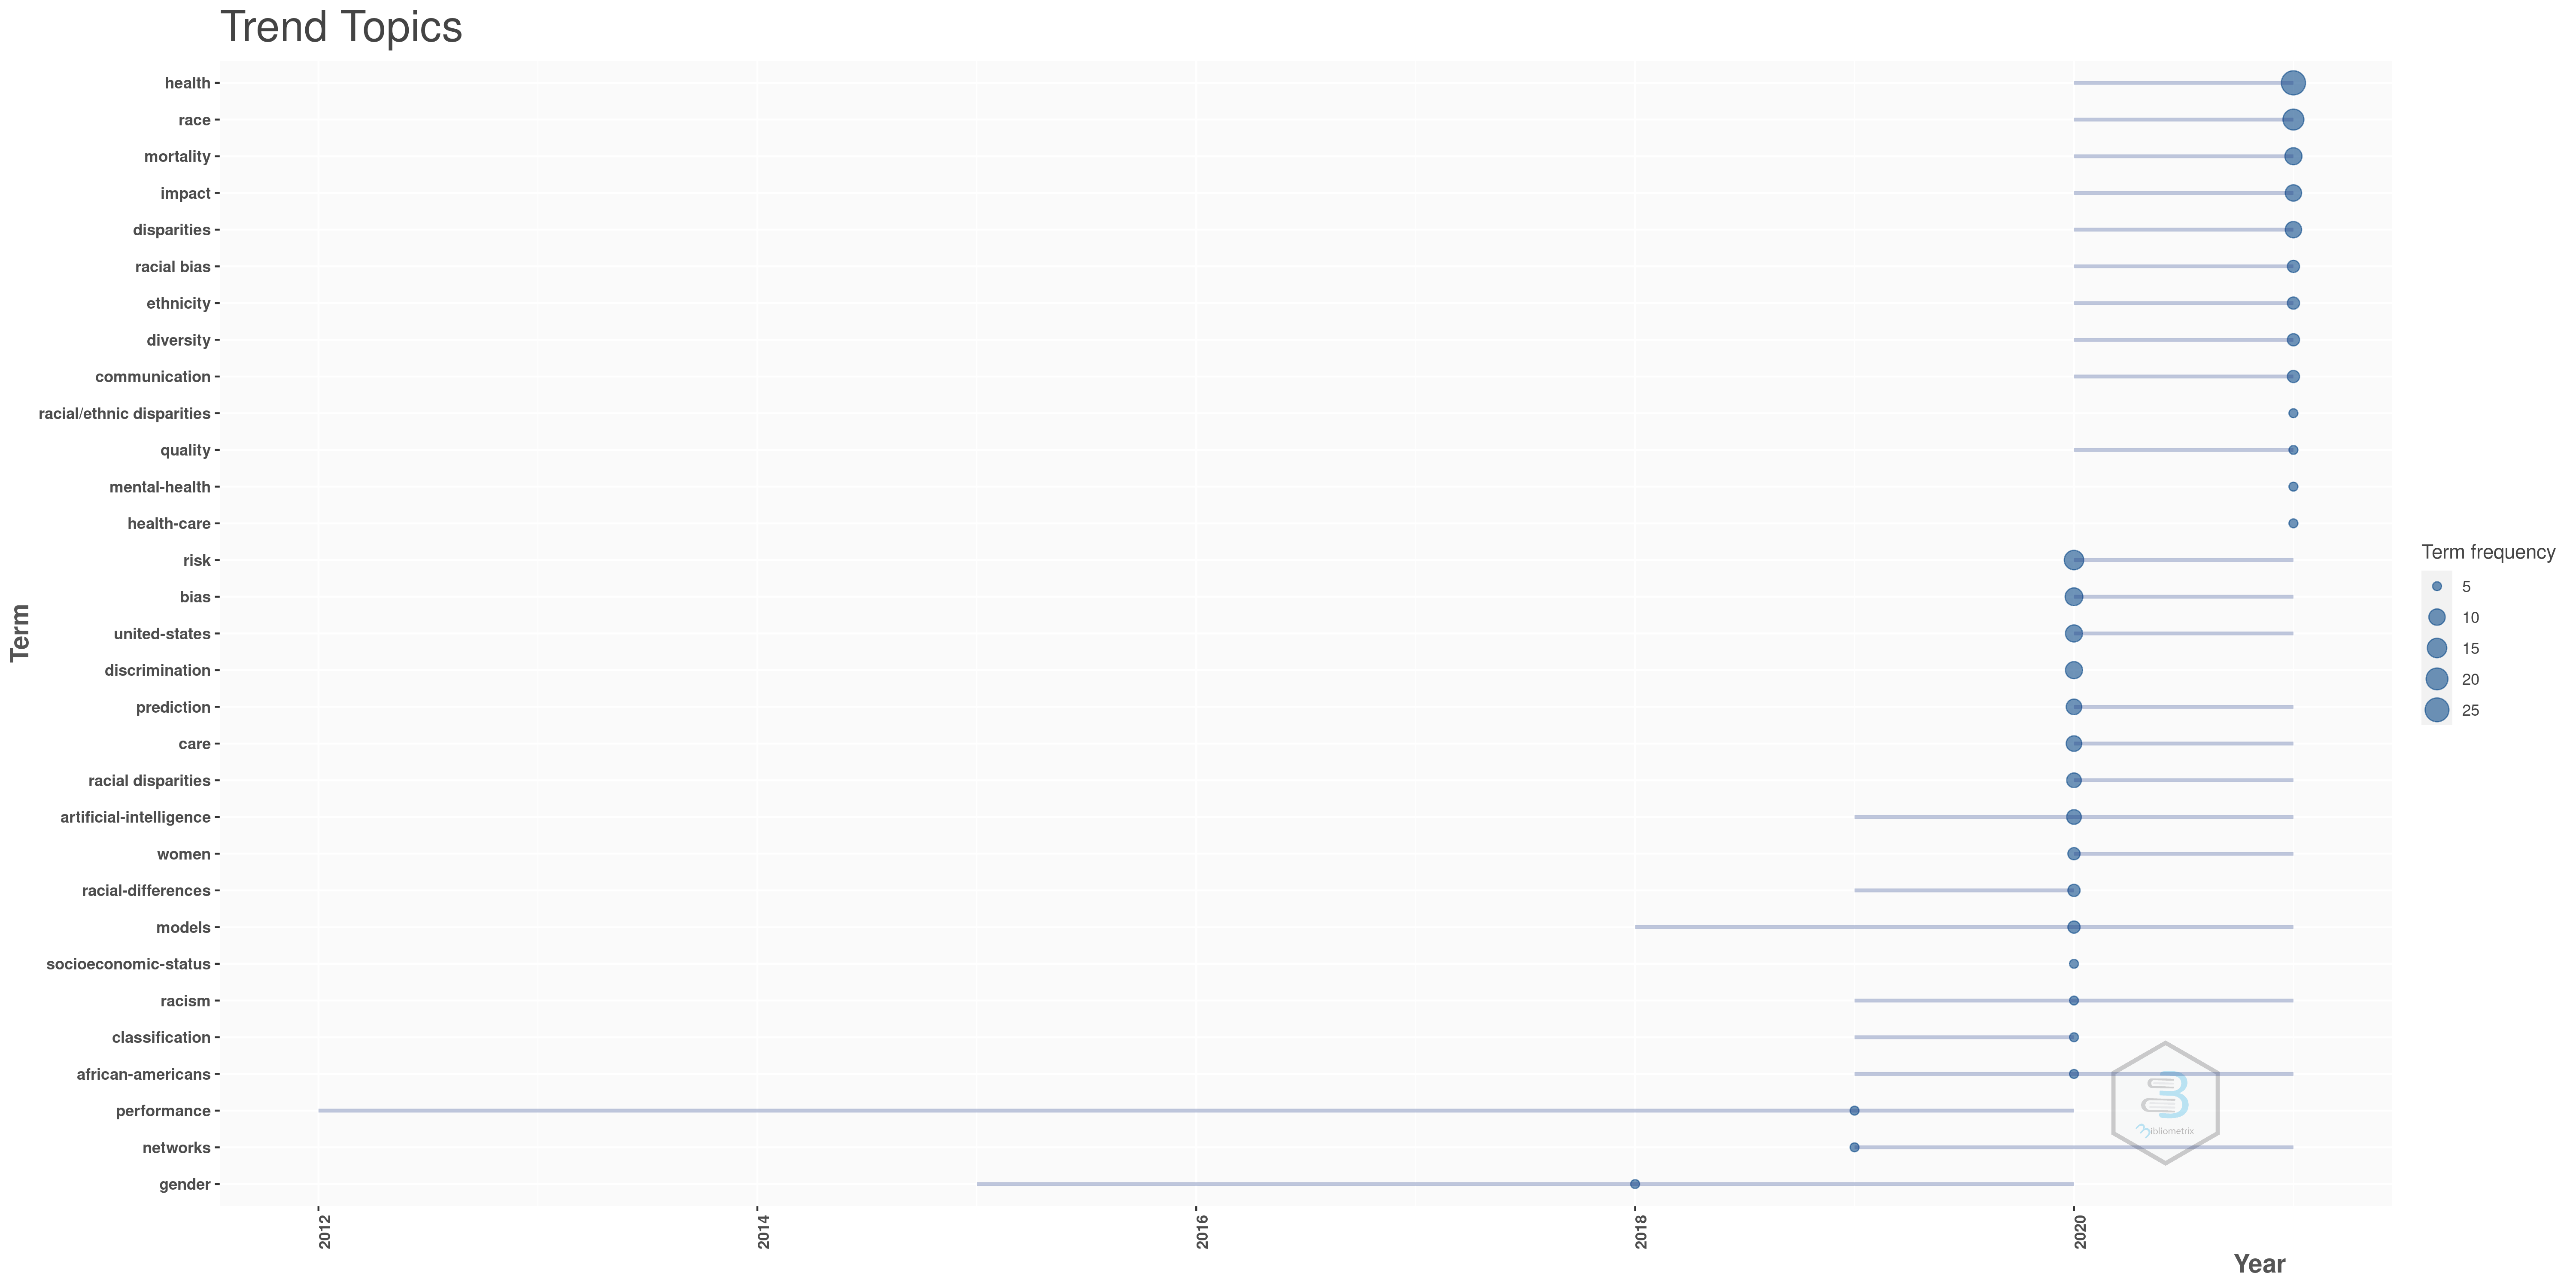
\includegraphics[angle=0,width=1\textwidth]{experiments/ngsylar/PesqBibliogr/Imagens/TrendTopics-2022-02-09.png}
    \caption{Tópicos de tendência do dataset ASADES@ngsylar.}
    \label{fig:ASADES@ngsylar:TT}
\end{figure}

A figura \ref{fig:ASADES@ngsylar:RelevantWords} mostra as 20 palavras mais relevantes dentro do contexto do conjunto de dados, extraíndo-as das \textit{Keywords Plus}. Dessa forma, podemos verificar o comportamento já apontado anteriormente, onde é visto o termo \textit{health (saúde)} indicando uma relação dos impactos negativos sobre as populações negras. Note a presença das palavras \textbf{risk (risco)}, \textbf{bias (viés)}, \textbf{discrimination (discriminação)}, \textbf{mortality (mortalidade)} \textbf{disparities (disparidades)}, \textbf{impact (impacto)}, são todas palavras negativas que representam a dimensão perigosa da aplicação da Inteligência Artificial.

Na figura \ref{fig:ASADES@ngsylar:TT}, vemos quando essas palavras se tornam tópicos em destaque, sendo consideradas tendências ou não. Inicialmente, vemos que quase não existem ensaios acadêmicos acerca da questão da discriminação e reforço de preconceitos através de algortimos de IA. Por volta de 2015, surge um ensaio envolvendo questões de gênero. Porém apenas em 2020, são discutidos os problemas do enviesamento dos algoritmos, os riscos e impactos advindos dessa problemática e saúde dos grupos étnicos atingidos. Posto isso, sabe-se que a área de IA vem se desenvolvendo desde o século passado porém é notável que na última década foi quando a Inteligência Artificial teve sua rápida expansão e ascensão. Logo, debates sobre diversidade, igualdade, ética e impactos que deveriam acompanhar a evolução deste artefato tecnológico estão sendo desenvolvidos somente agora, com quase uma década de atraso. 


\subsubsection{Agrupamento}

Podemos realizar o agrupamento dos documentos em \textit{clusters}, serão agrupados artigos utilizando a métrica de Palavras-chave do Autor, além disso é medido também o impacto desses clusters utilizando o Impacto Global dos Artigos. Dessa forma na figura \ref{fig:ASADES@ngsylar:Coupling}, abaixo, notamos a presença dos grupos acerca, aqui podemos comprovar que apesar de estarem relacionados --- veja o eixo horizontal, ambos possuem valores baixos de relevância, indicando uma baixa relação --- com tema eles tem baixo impacto --- basta ver o eixo horizontal, ambos também possuem valores baixos de impacto.

O grupos importantes estão mais à direita do gráfico, podemos ver que o grupo vermelho possui um alto impacto o que faz sentido uma vez que é uma das cláusulas principais do estudo. Por outro lado, o grupo verde tem alta relevância como o tema o que também faz sentido pois essa é a outra cláusula do estudo. O grupo amarelo se aproxima mais ao verde, pois não trata da discriminação racial por meios implementados com AI e sim como usar IA para identificar essas agressões. 

\begin{figure}
    \centering
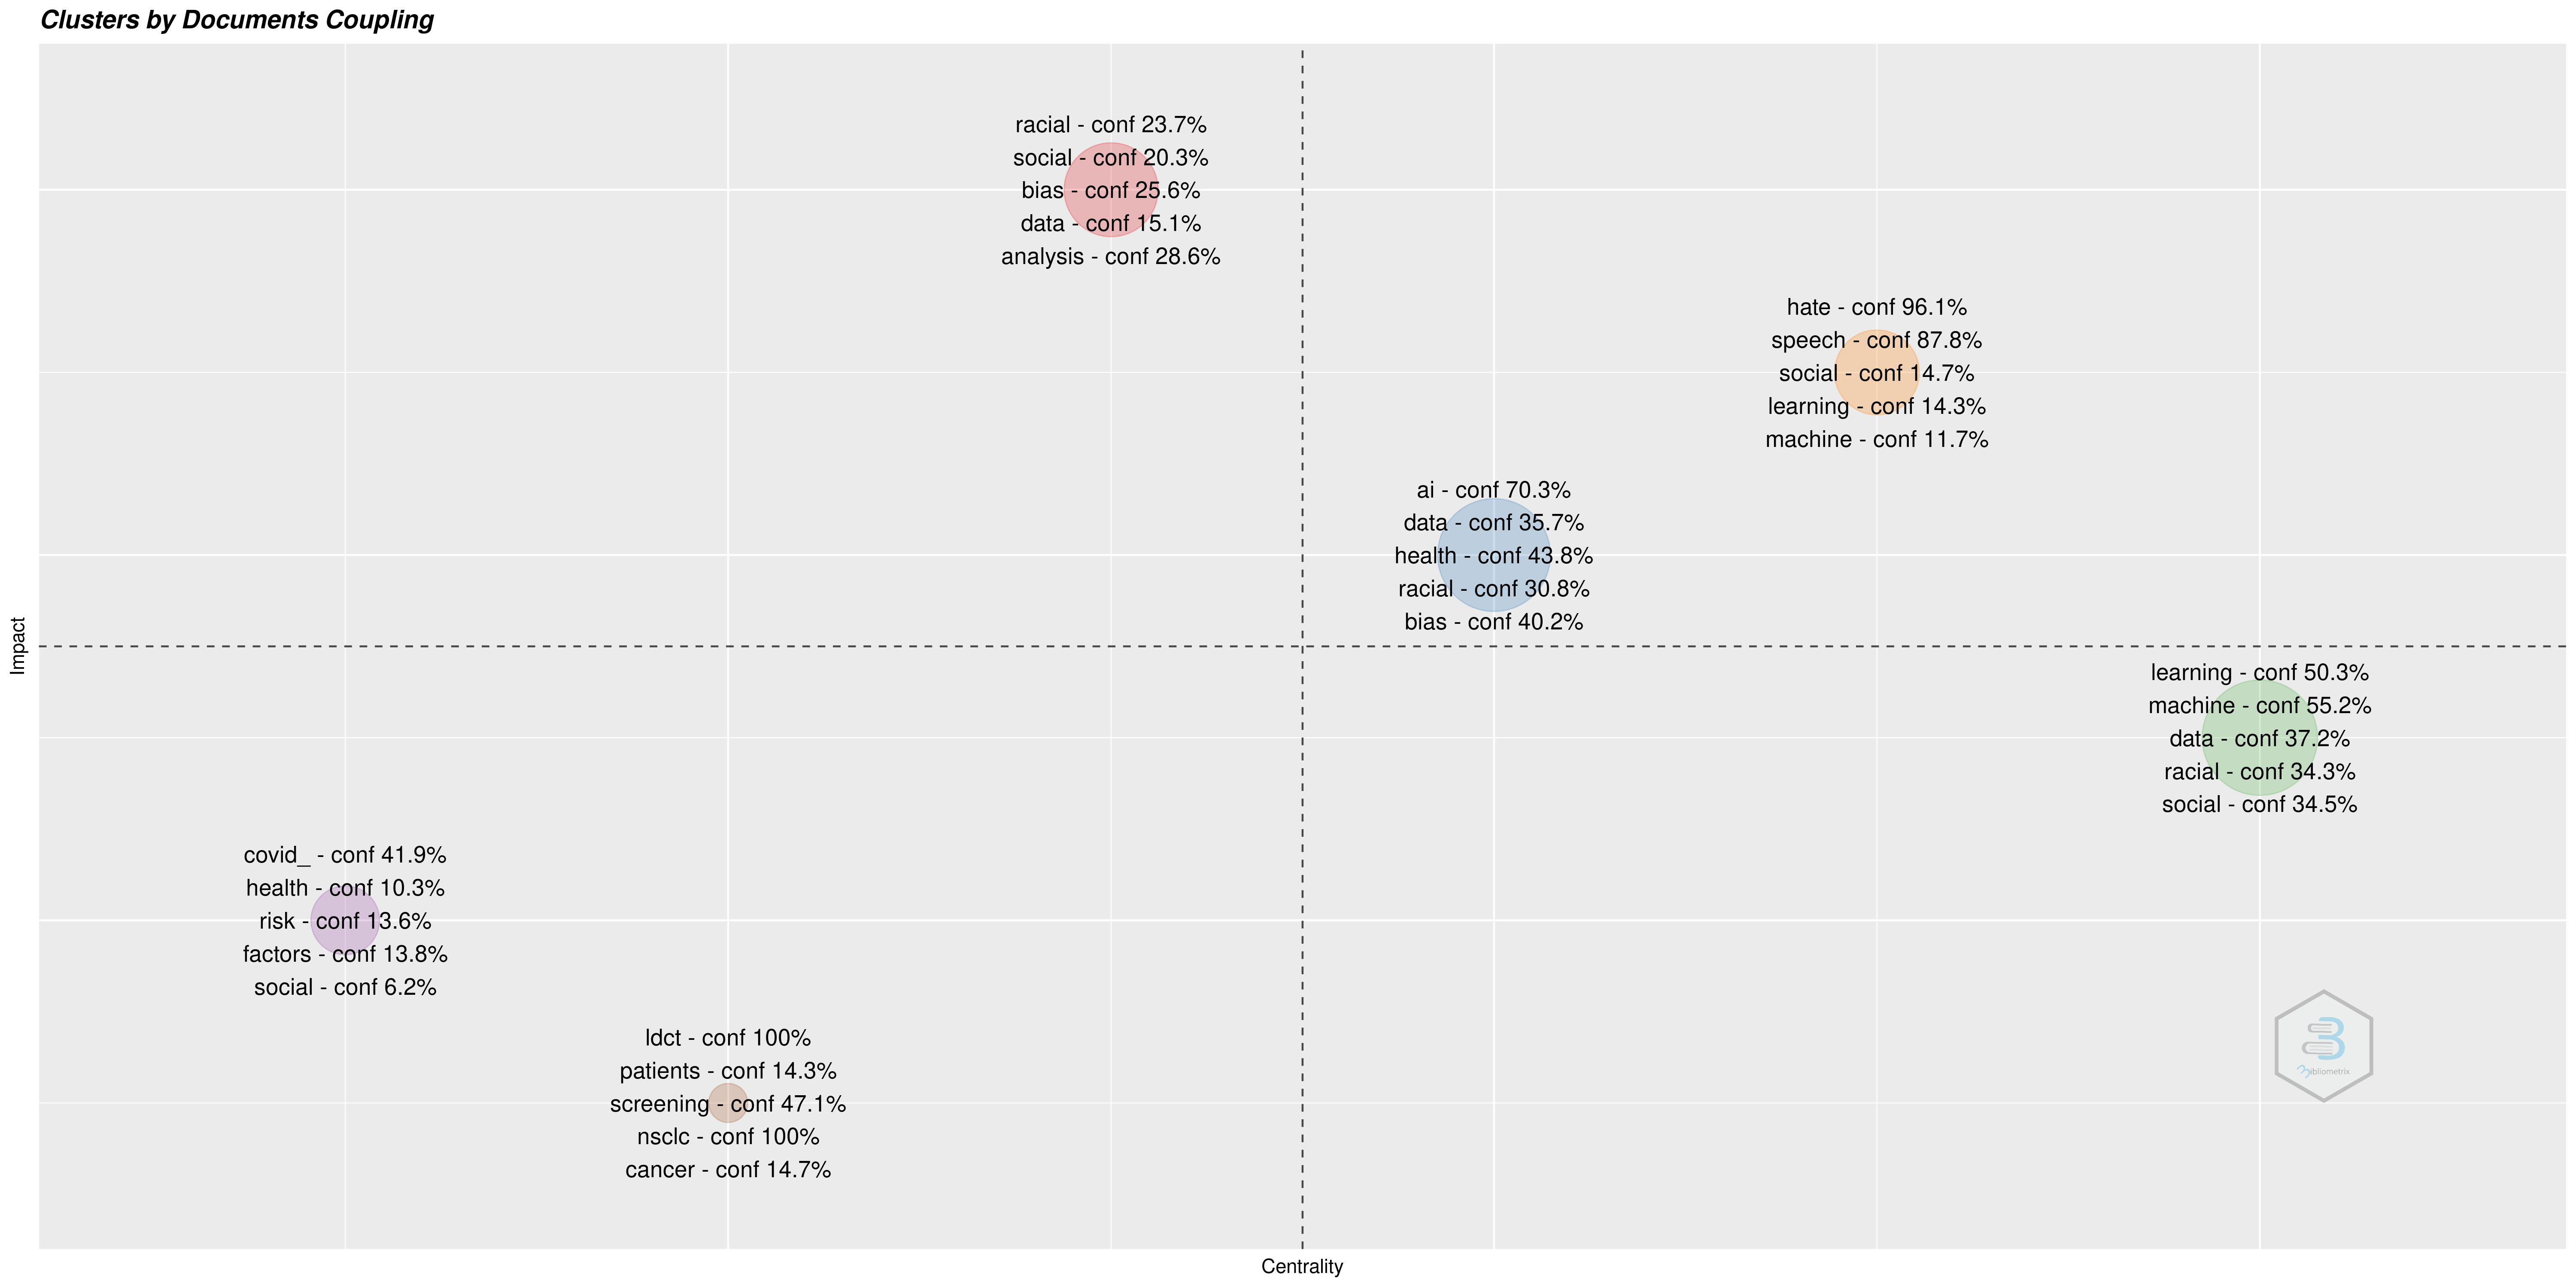
\includegraphics[angle=0,width=1\textwidth]{experiments/ngsylar/PesqBibliogr/Imagens/CouplingMap-2022-02-09.png}
    \caption{Agrupamento dos Documentos do dataset ASADES@ngsylar.}
    \label{fig:ASADES@ngsylar:Coupling}
\end{figure}


\subsection{Estrutura Conceitual}

\subsubsection{Coocorrência de Keywords Plus}

\begin{figure}
    \centering
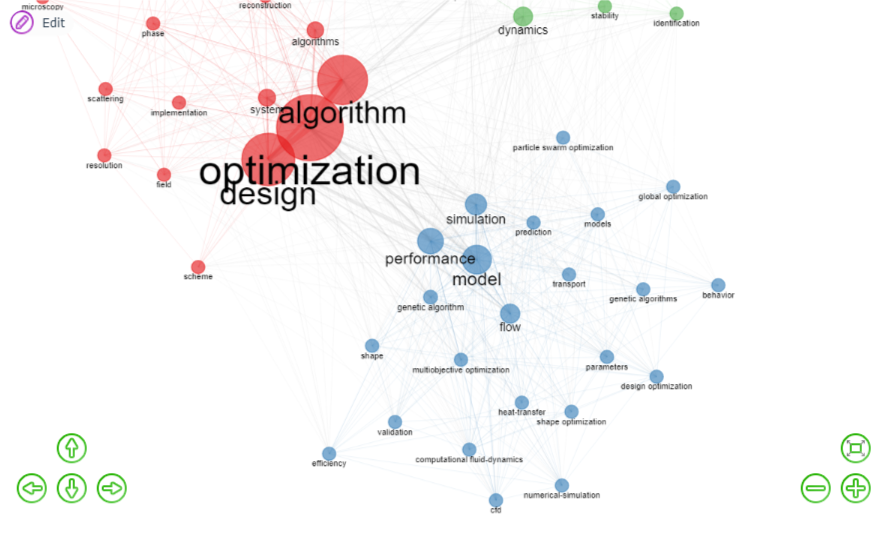
\includegraphics[angle=0,width=1\textwidth]{experiments/ngsylar/PesqBibliogr/Imagens/CoOccurrence.png}
    \caption{Rede de coocorrência de Keywords Plus do dataset ASADES@ngsylar.}
    \label{fig:ASADES@ngsylar:CoOcorrenceKW}
\end{figure}

De acordo com a figura \ref{fig:ASADES@ngsylar:CoOcorrenceKW} podemos visualizar de uma forma mais intuitiva as palavras que aparecem simultâneamente nas Keywords Plus dos artigos, vemos aqui claramente o quão nocivo são os algortimos de IA enviesados e os riscos que eles apresentam para a população negra.

\subsubsection{Mapa temático}
\begin{figure}[H]
    \centering
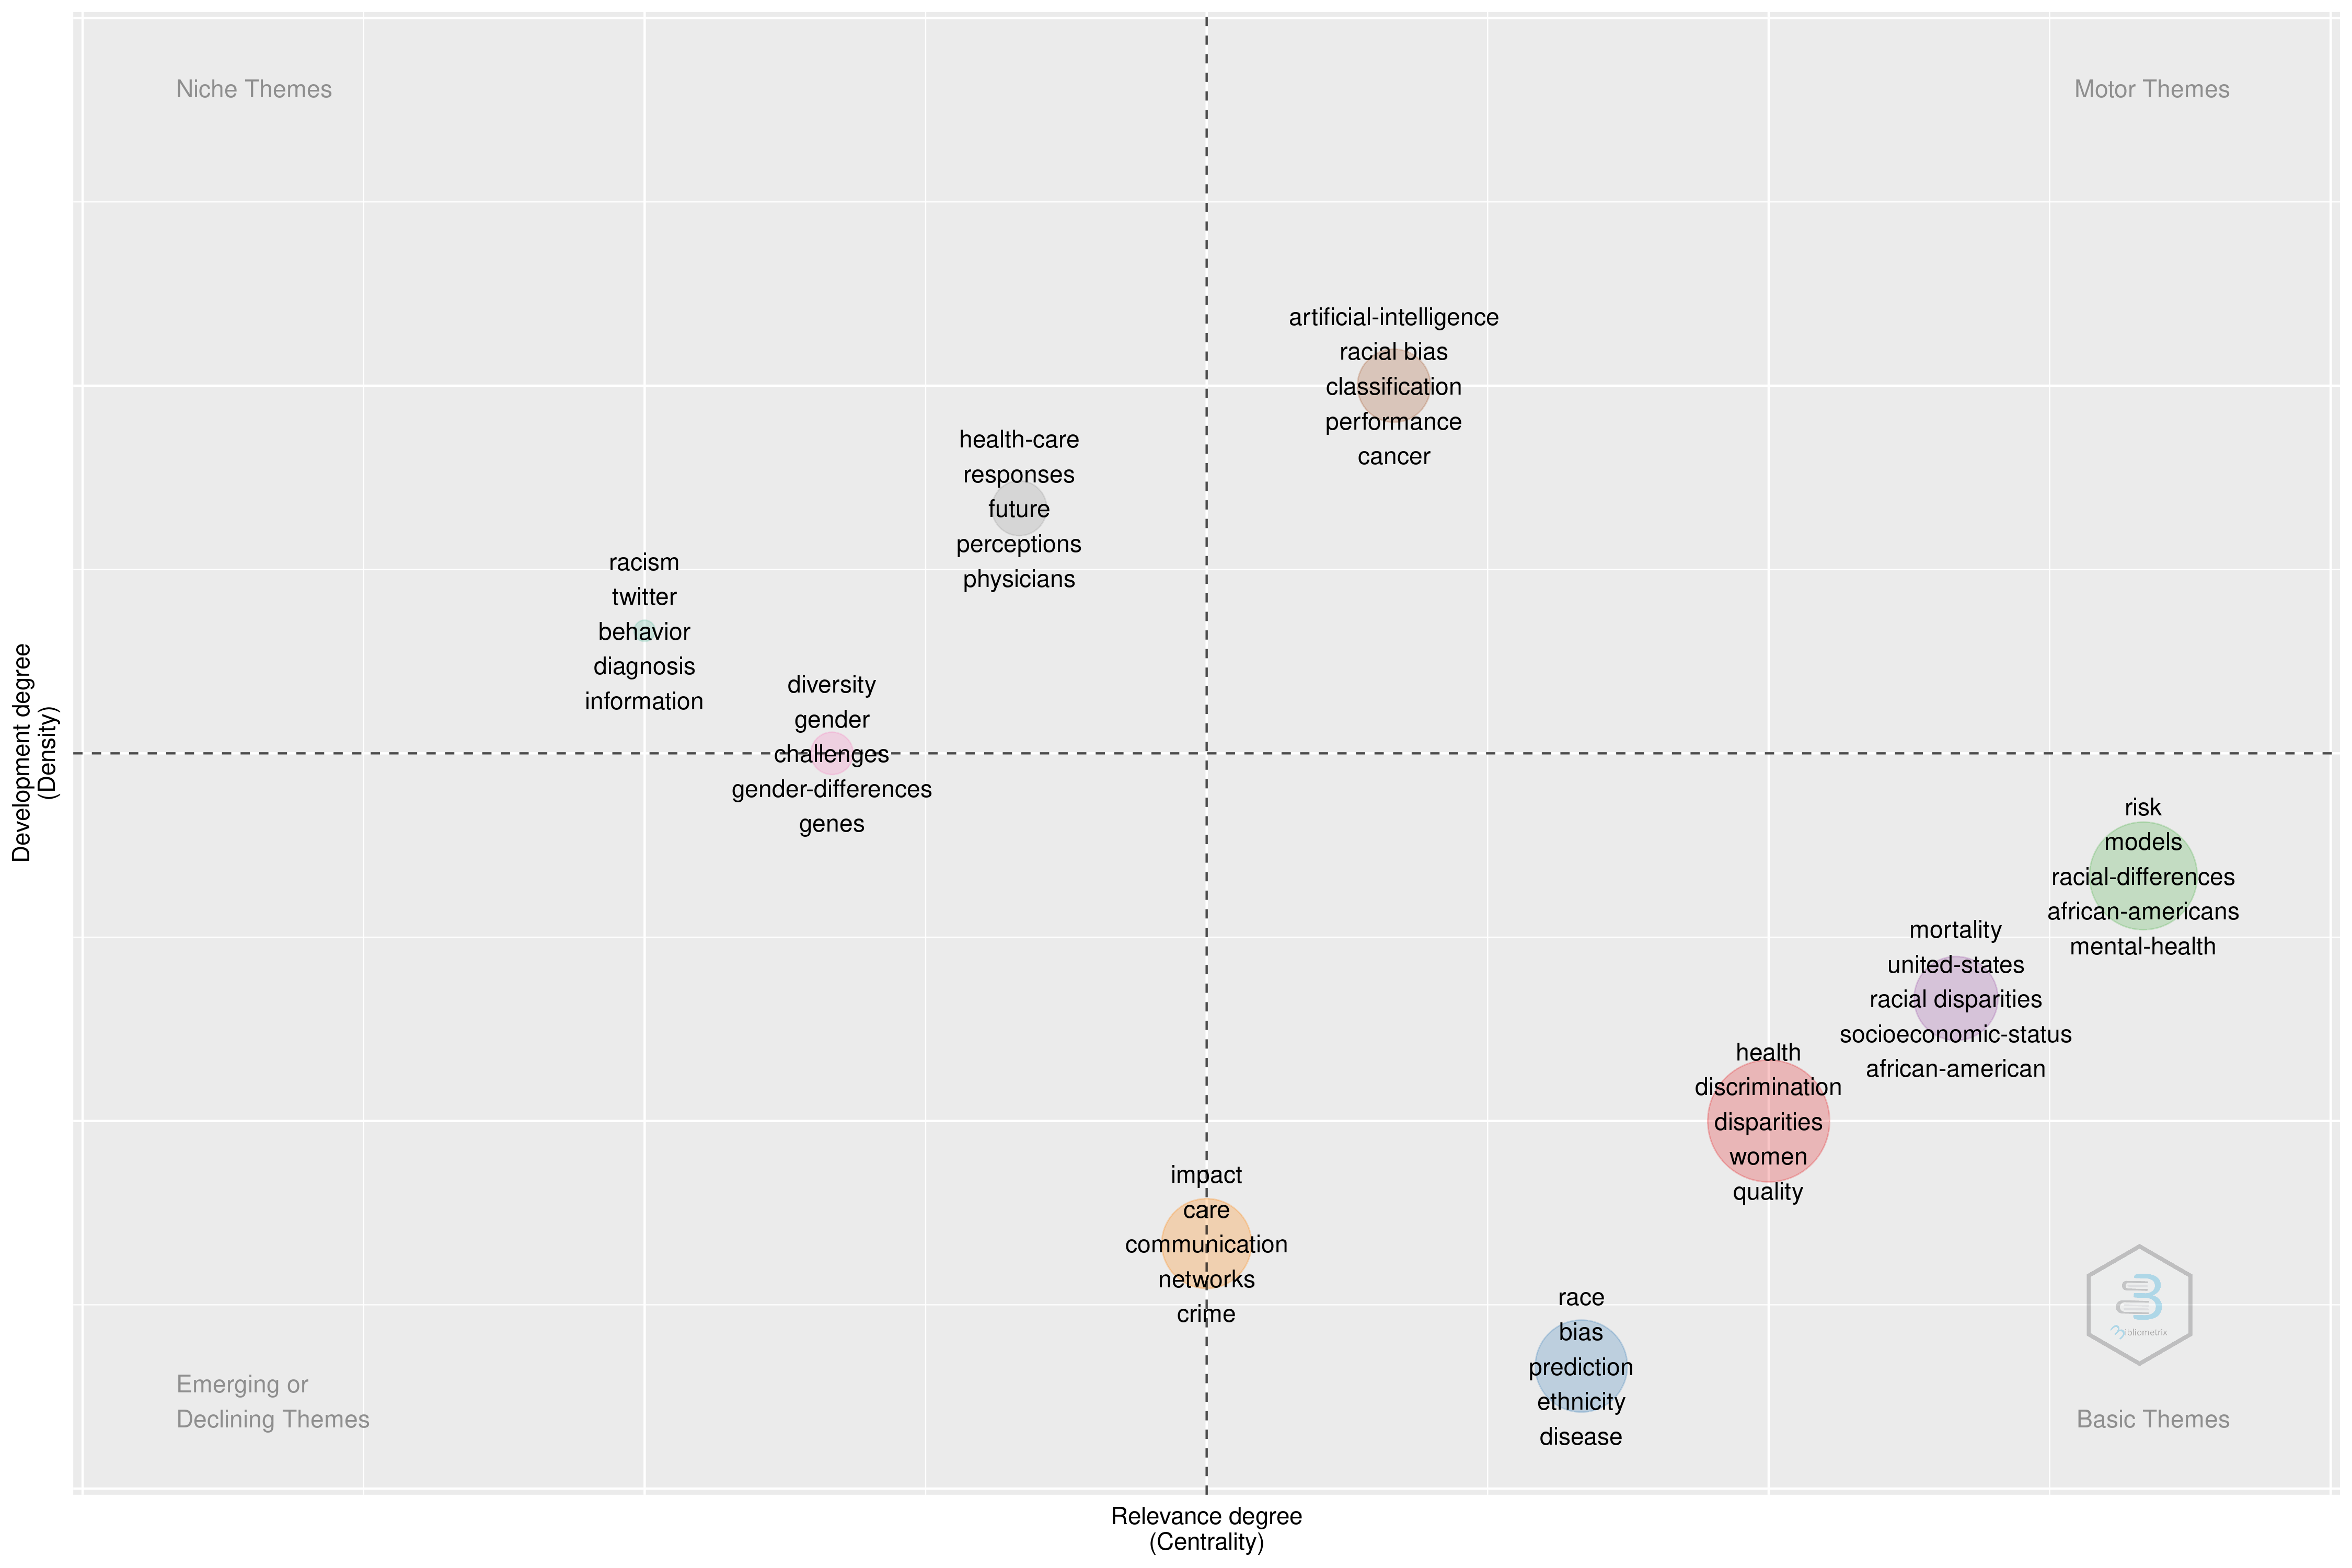
\includegraphics[angle=0,width=1\textwidth]{experiments/ngsylar/PesqBibliogr/Imagens/ThematicMap-2022-02-09.png}
    \caption{Mapa temático do dataset ASADES@ngsylar.}
    \label{fig:ASADES@ngsylar:ThematicMap}
\end{figure}


Além disso podemos ver na figura \ref{fig:ASADES@ngsylar:ThematicMap}, do mapa temático, essas mesmas Keywords agrupadas formando temas. 

Observa-se que há temas --- cinza, rosa e ciano --- que não possuem uma relevância tão alta para o estudo porém indicam um nível maior de desenvolvimento. Enquanto isso, os temas centrais do estudo, os que estão mais à direita, possuem um baixo grau de desenvolvimento. Dessa forma, essa imagem comprova o baixo aprofundamento nas questões centrais desse estudo.

O grupo marrom mostra que já há um certo nível de entendimento da necessidade de se atentar ao critério racial no que se diz respeito ao uso de IA para uma boa performance na classificação do diagnóstico de cancer. 

\subsubsection{Mapa fatorial}
\begin{figure}[H]
    \centering
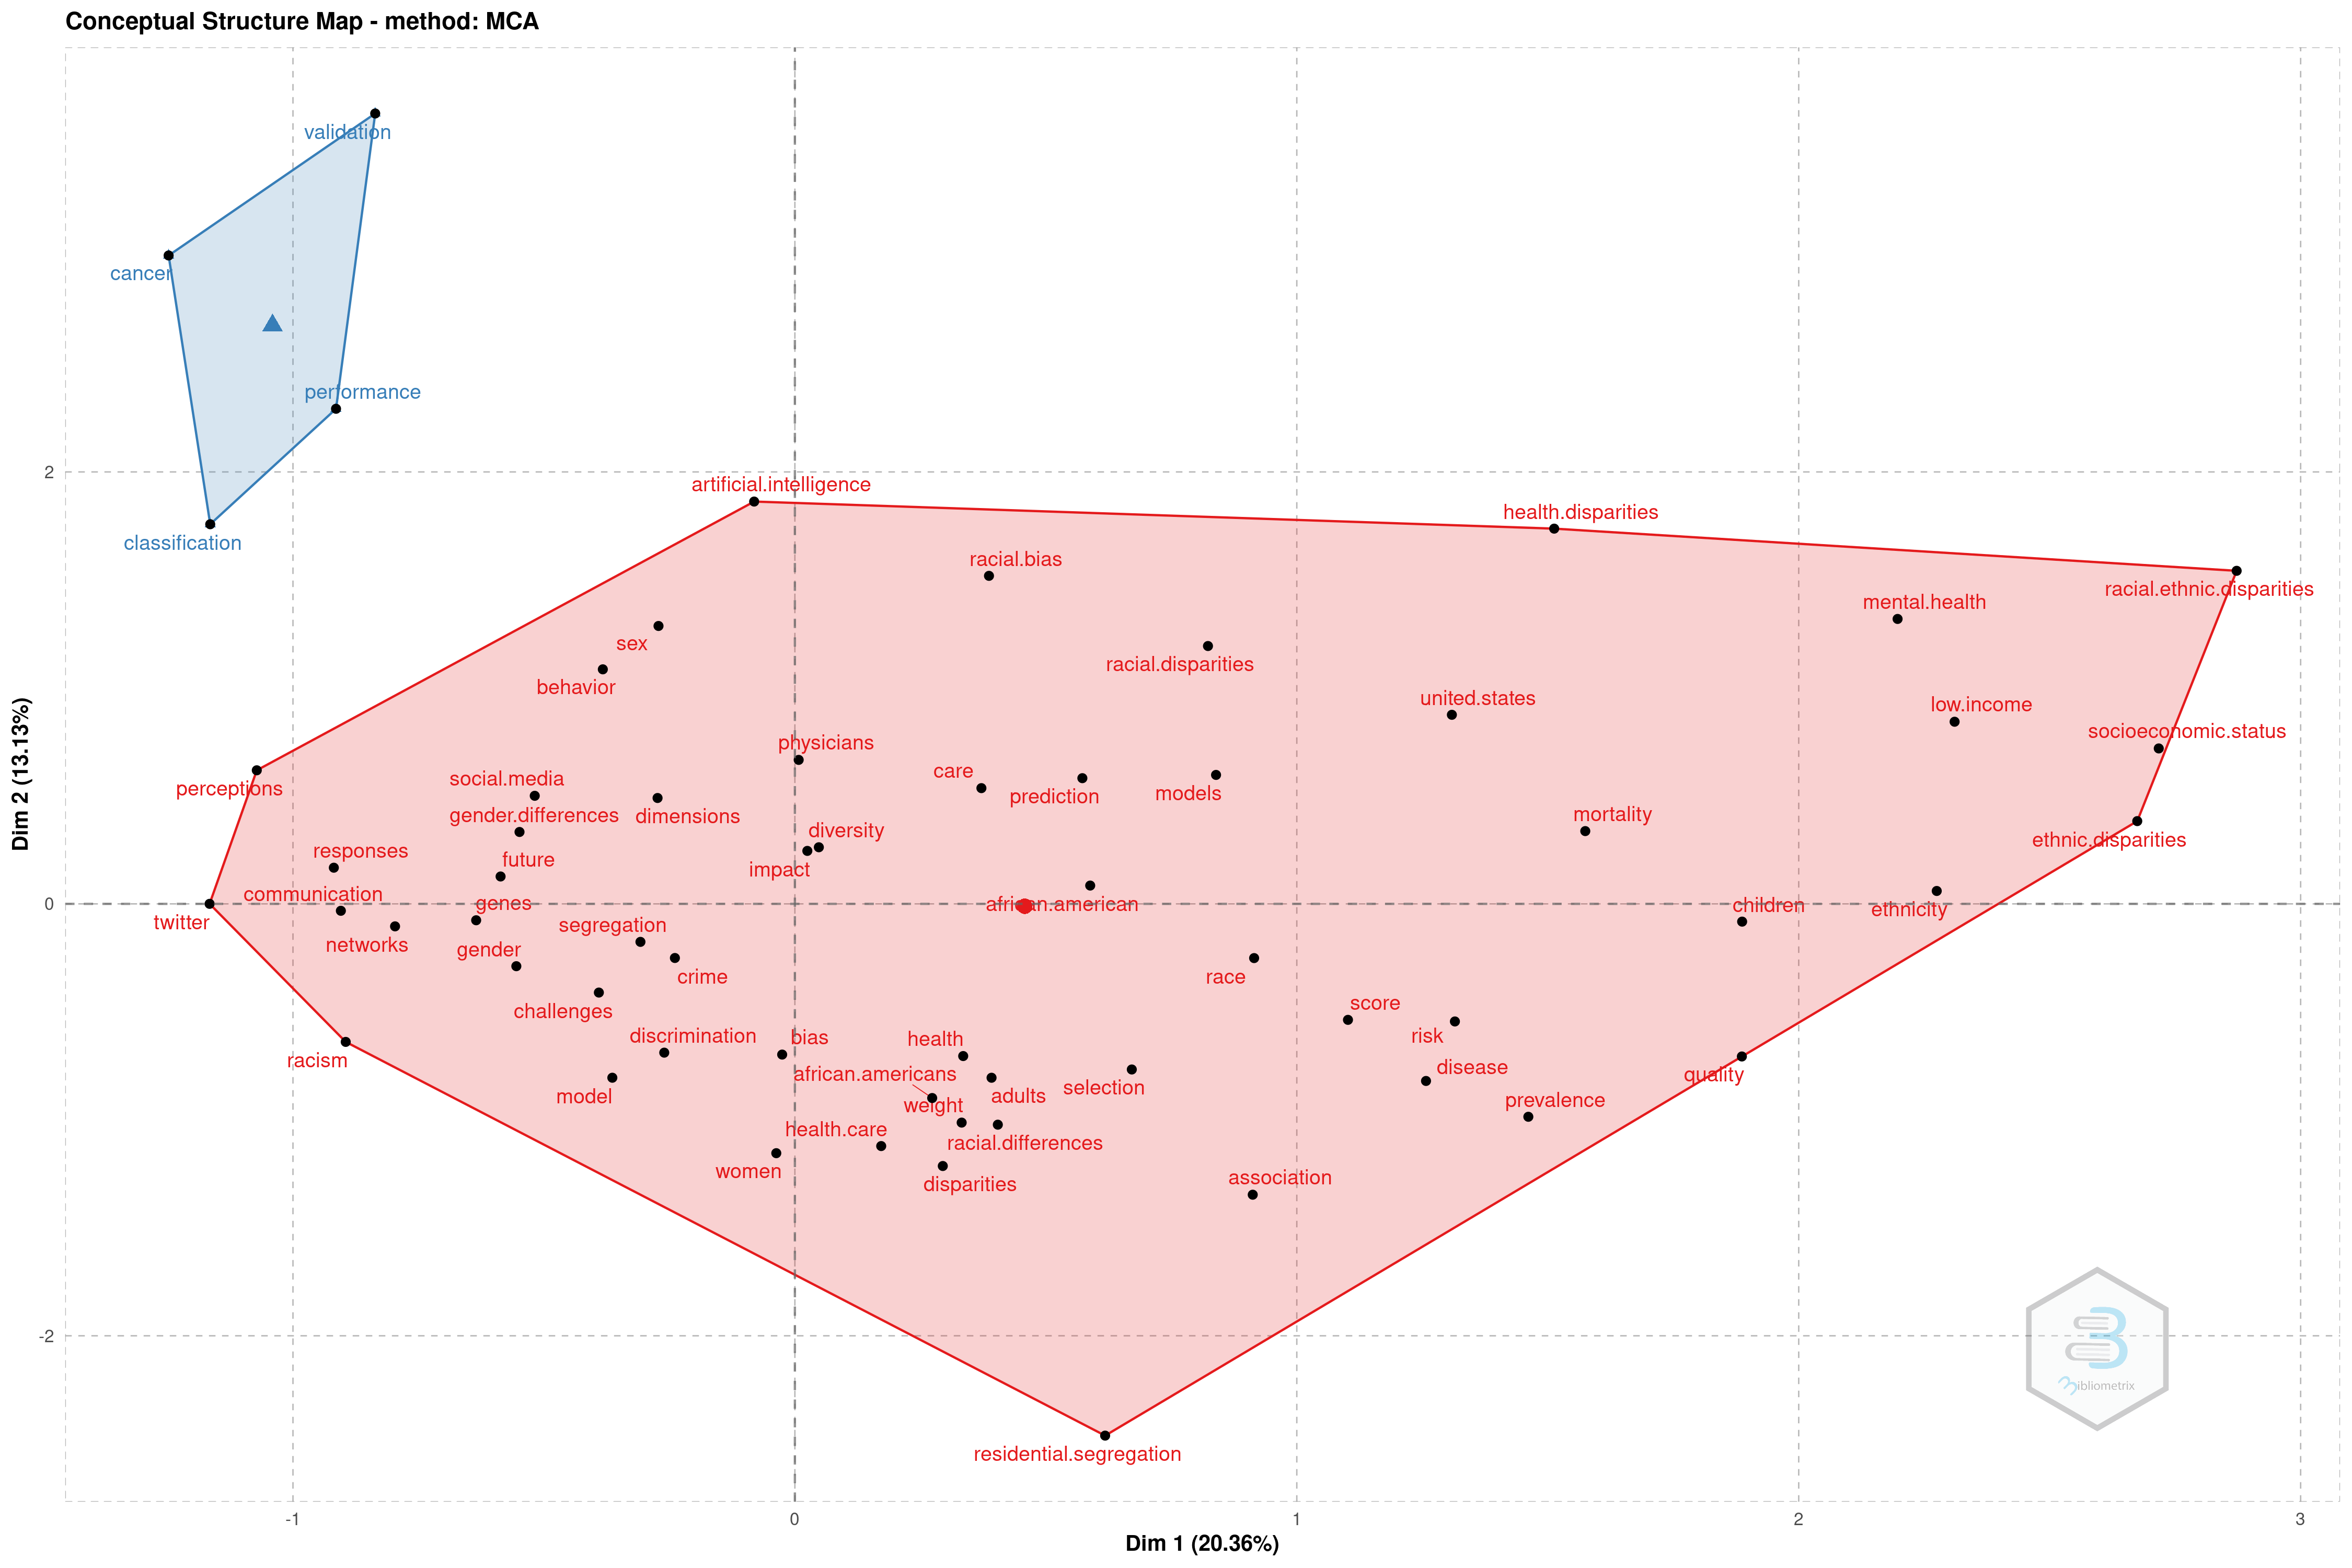
\includegraphics[angle=0,width=1\textwidth]{experiments/ngsylar/PesqBibliogr/Imagens/FactorialMap-2022-02-09.png}
    \caption{Mapa fatorial das Keywords Plus do dataset ASADES@ngsylar.}
    \label{fig:ASADES@ngsylar:FactorialMap}
\end{figure}

\begin{figure}[H]
    \centering
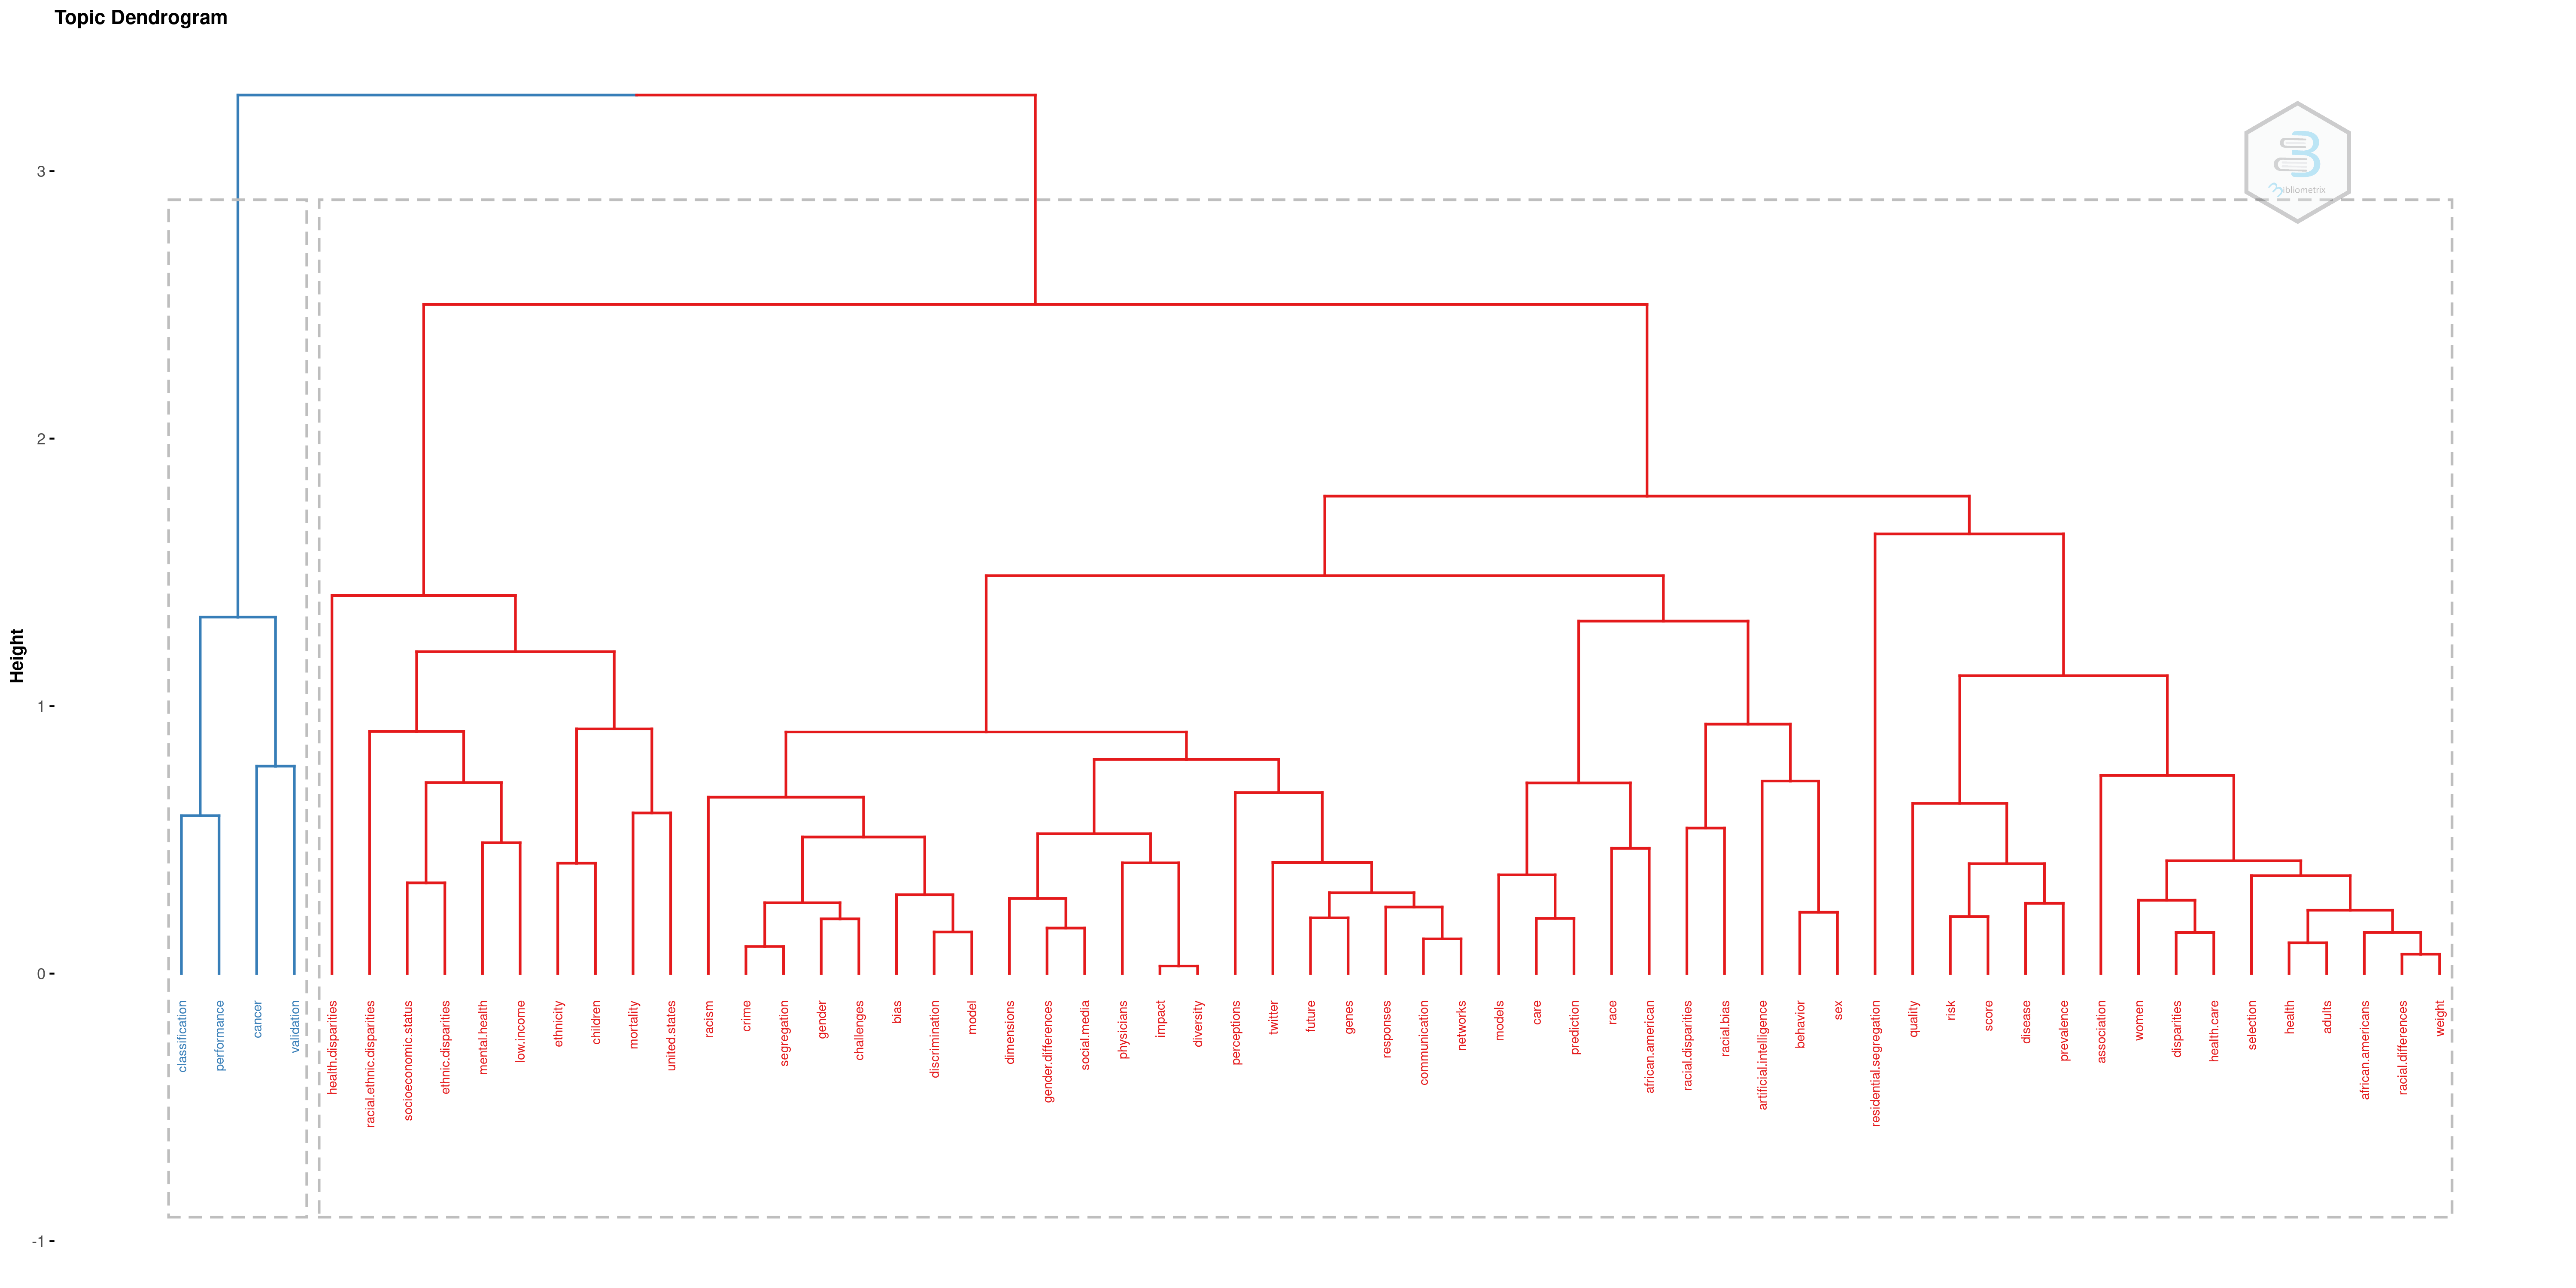
\includegraphics[angle=0,width=1\textwidth]{experiments/ngsylar/PesqBibliogr/Imagens/Dendrogram-2022-02-09.png}
    \caption{Dendeograma das Keywords Plus do dataset ASADES@ngsylar.}
    \label{fig:ASADES@ngsylar:Dendeogram}
\end{figure}


Utilizando novamente a métrica das Keywords Plus, podemos ver que nessa figura \ref{fig:ASADES@ngsylar:FactorialMap} há dois grandes grupos do conhecimento, sendo o maior deles, em vermelho, mais interessado em dialogar sobre questões étnicas, raciais e enviesamento dentro da área da Inteligência Artificial. O outro, menor, em azul, enfatiza a questão da classificação de diagnóstico de câncer utilizando IA. 

Na figura \ref{fig:ASADES@ngsylar:Dendeogram} podemos entender melhor como esses termos se interligam e visualizar a o quão relacionados eles estão, bem como, visualizar também o momento onde deixaram de se relacionar.


\subsection{Estrutura Intelectual}

\subsubsection{Rede de cocitação}

\begin{figure}[H]
    \centering
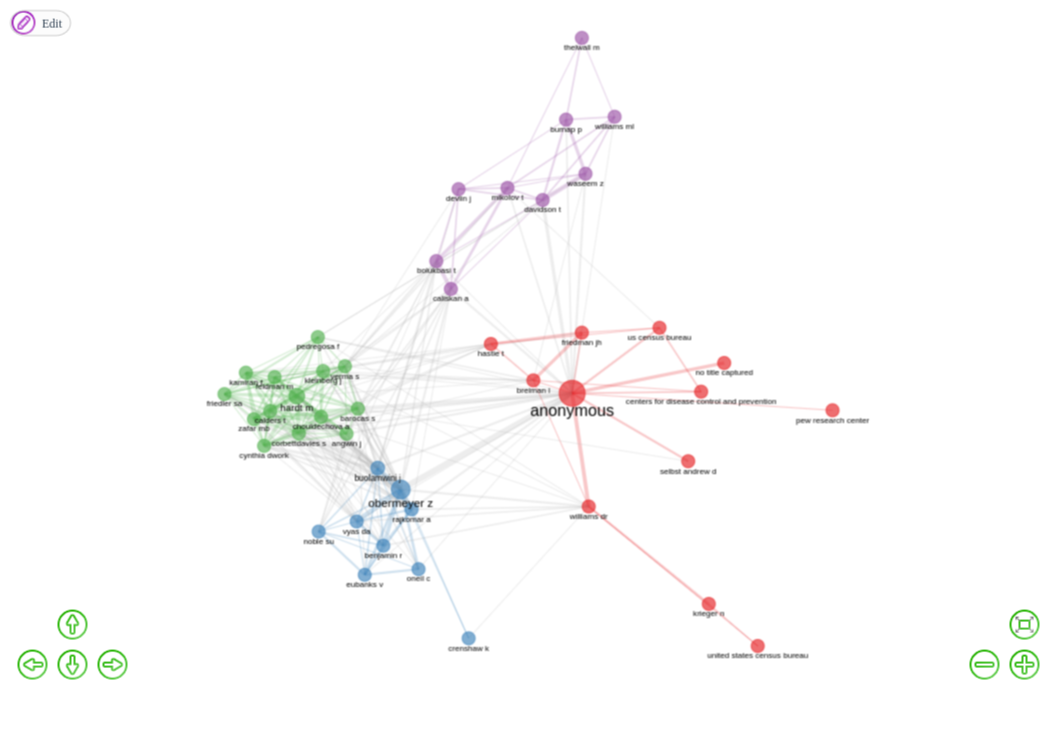
\includegraphics[angle=0,width=1\textwidth]{experiments/ngsylar/PesqBibliogr/Imagens/CoCitation.png}
    \caption{Rede de cocitação de Autores do dataset ASADES@ngsylar.}
    \label{fig:ASADES@ngsylar:Cocitation}
\end{figure}

De acordo com a figura \ref{fig:ASADES@ngsylar:Cocitation} podemos visualizar de uma forma mais intuitiva os autores que são citados simultâneamente, é possível ver que há vários núcleos onde os autores aparecem conjuntamente porém em cada um desses grupos há um autor em específico que aparece e se relaciona mais com os grupos externos ao dele.

\subsubsection{Historiografia}
\begin{figure}[H]
    \centering
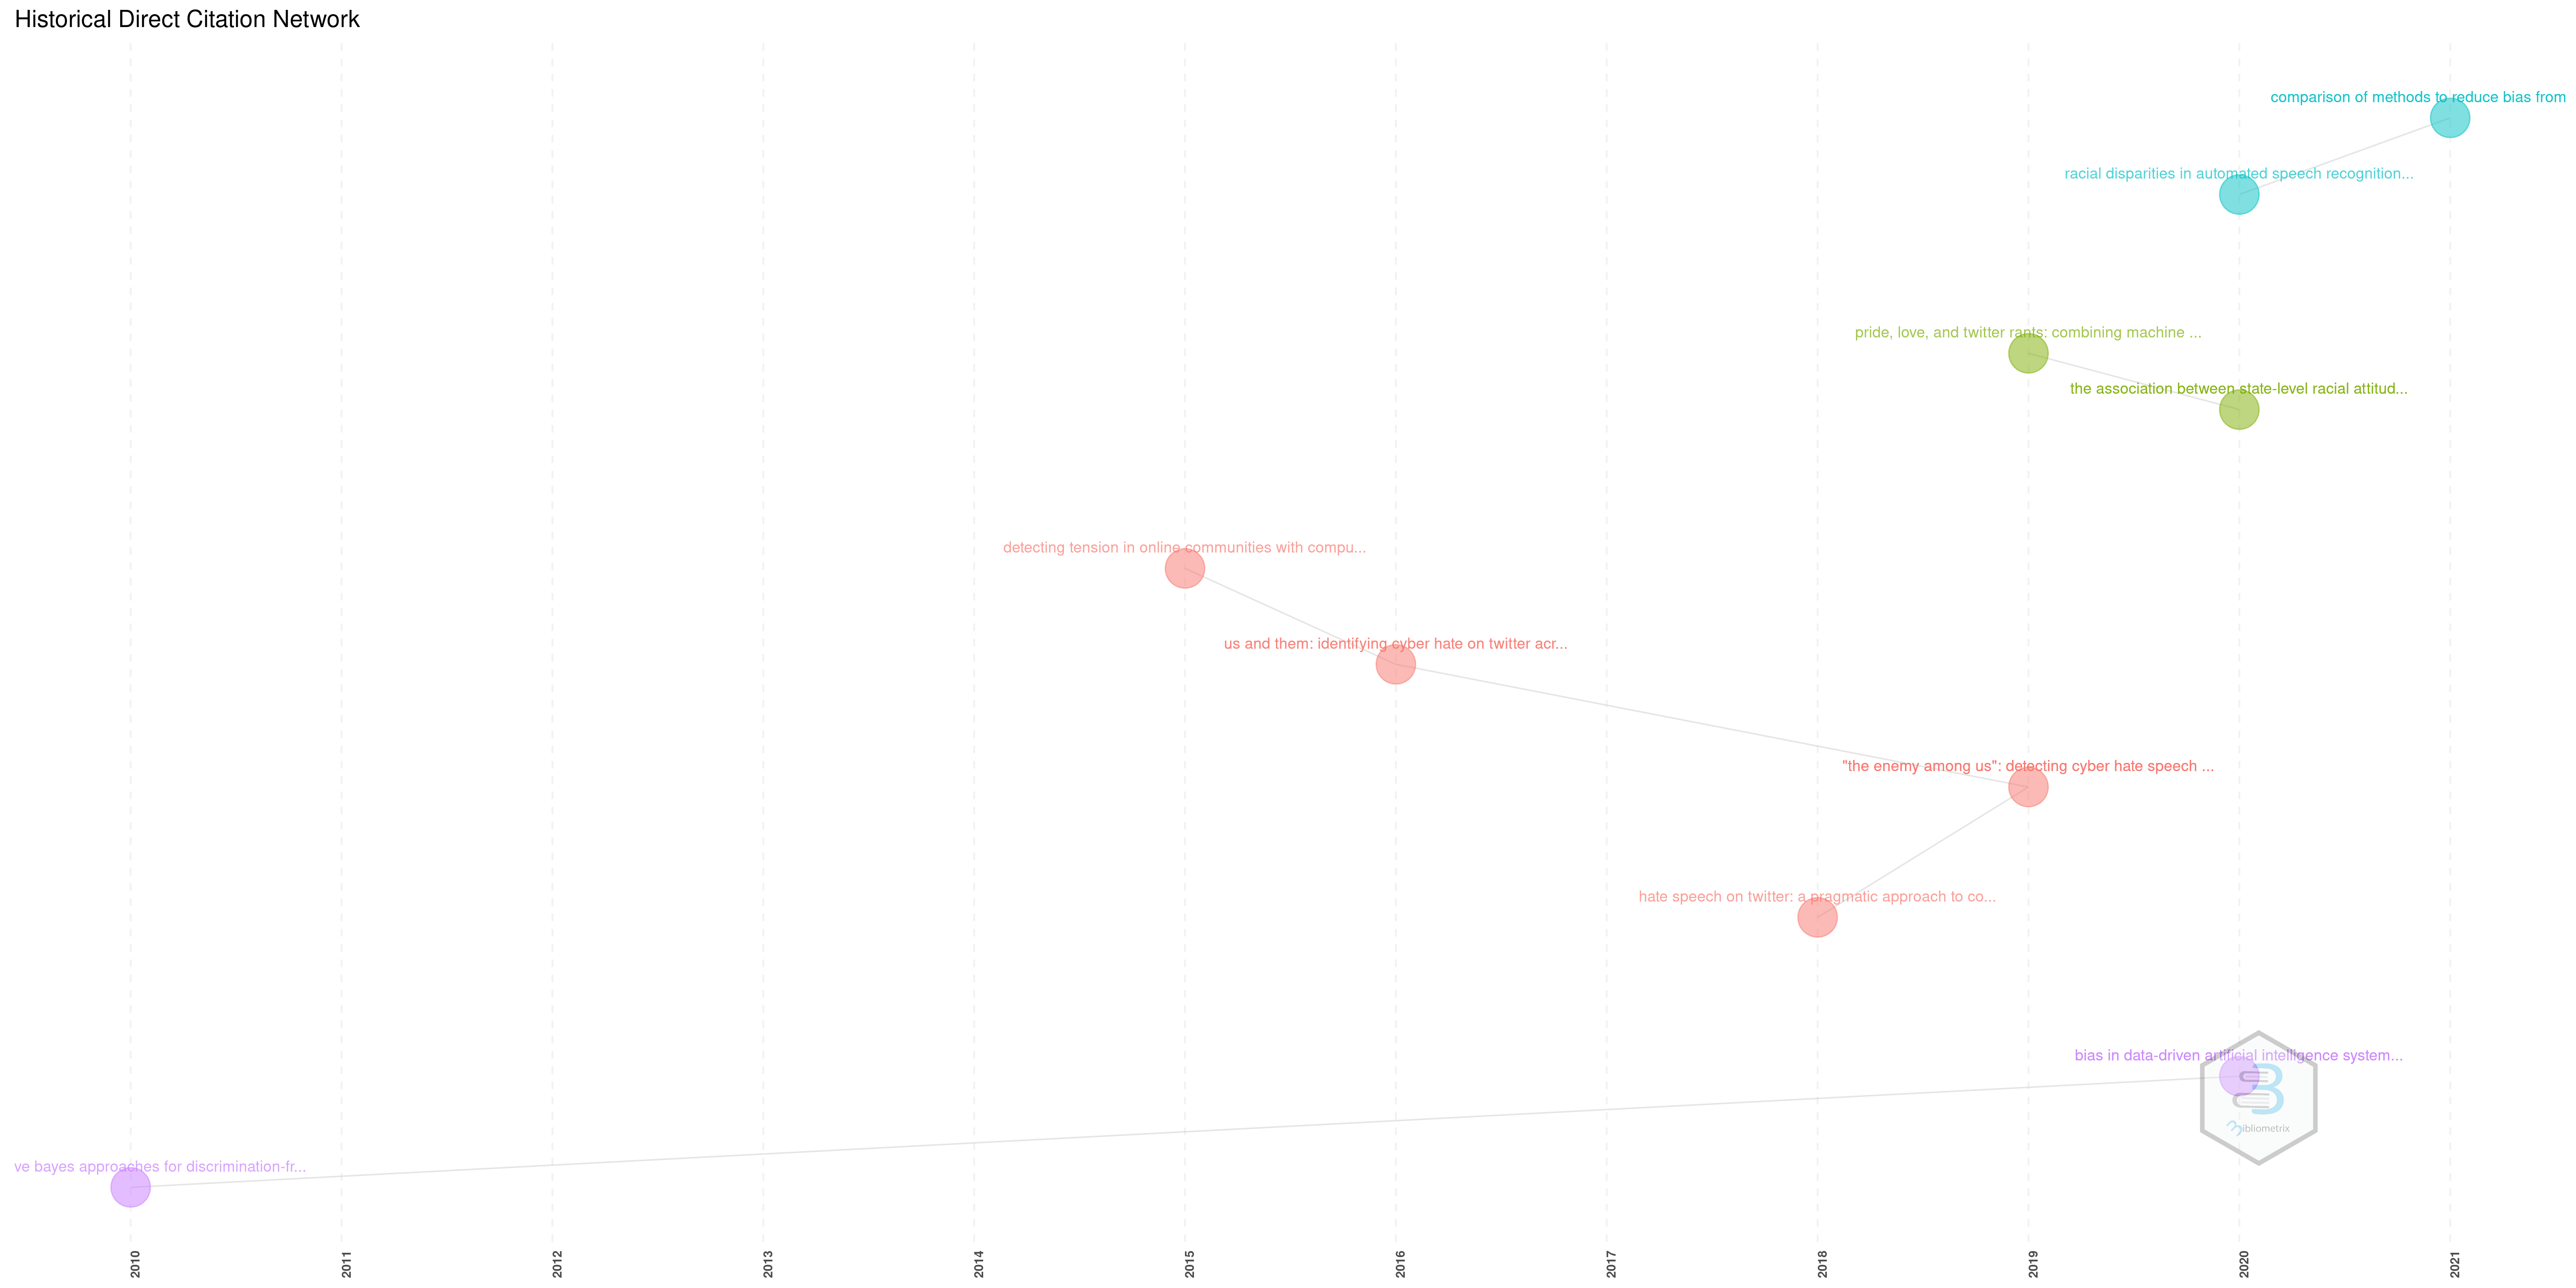
\includegraphics[angle=0,width=1\textwidth]{experiments/ngsylar/PesqBibliogr/Imagens/Historiograph-2022-02-09.png}
    \caption{Historiografia das cocitações do dataset ASADES@ngsylar.}
    \label{fig:ASADES@ngsylar:Historiograph}
\end{figure}

Na imagem \ref{fig:ASADES@ngsylar:Historiograph} podemos ver ao longo dos anos quais são os 20 artigos que mais citados e quais são os outros artigos que aparecem citados  conjuntamente à ele. 

Vemos um grupo que foge um pouco do escopo --- trata-se de identificação de discursos de ódio nas redes sociais -- porém os outros todos são relativos ao tópico central deste presente estudo. Sendo explicado o baixo número de cocitação em razão de que, como vimos na secção anterior, em geral, artigos de um mesmo grupo acabam sendo mais citados conjuntamente do que com outros artigos que escapam deste grupo.


\subsection{Estrutura Social}

\subsubsection{Mapa mundial das Colaborações}

\begin{figure}[H]
    \centering
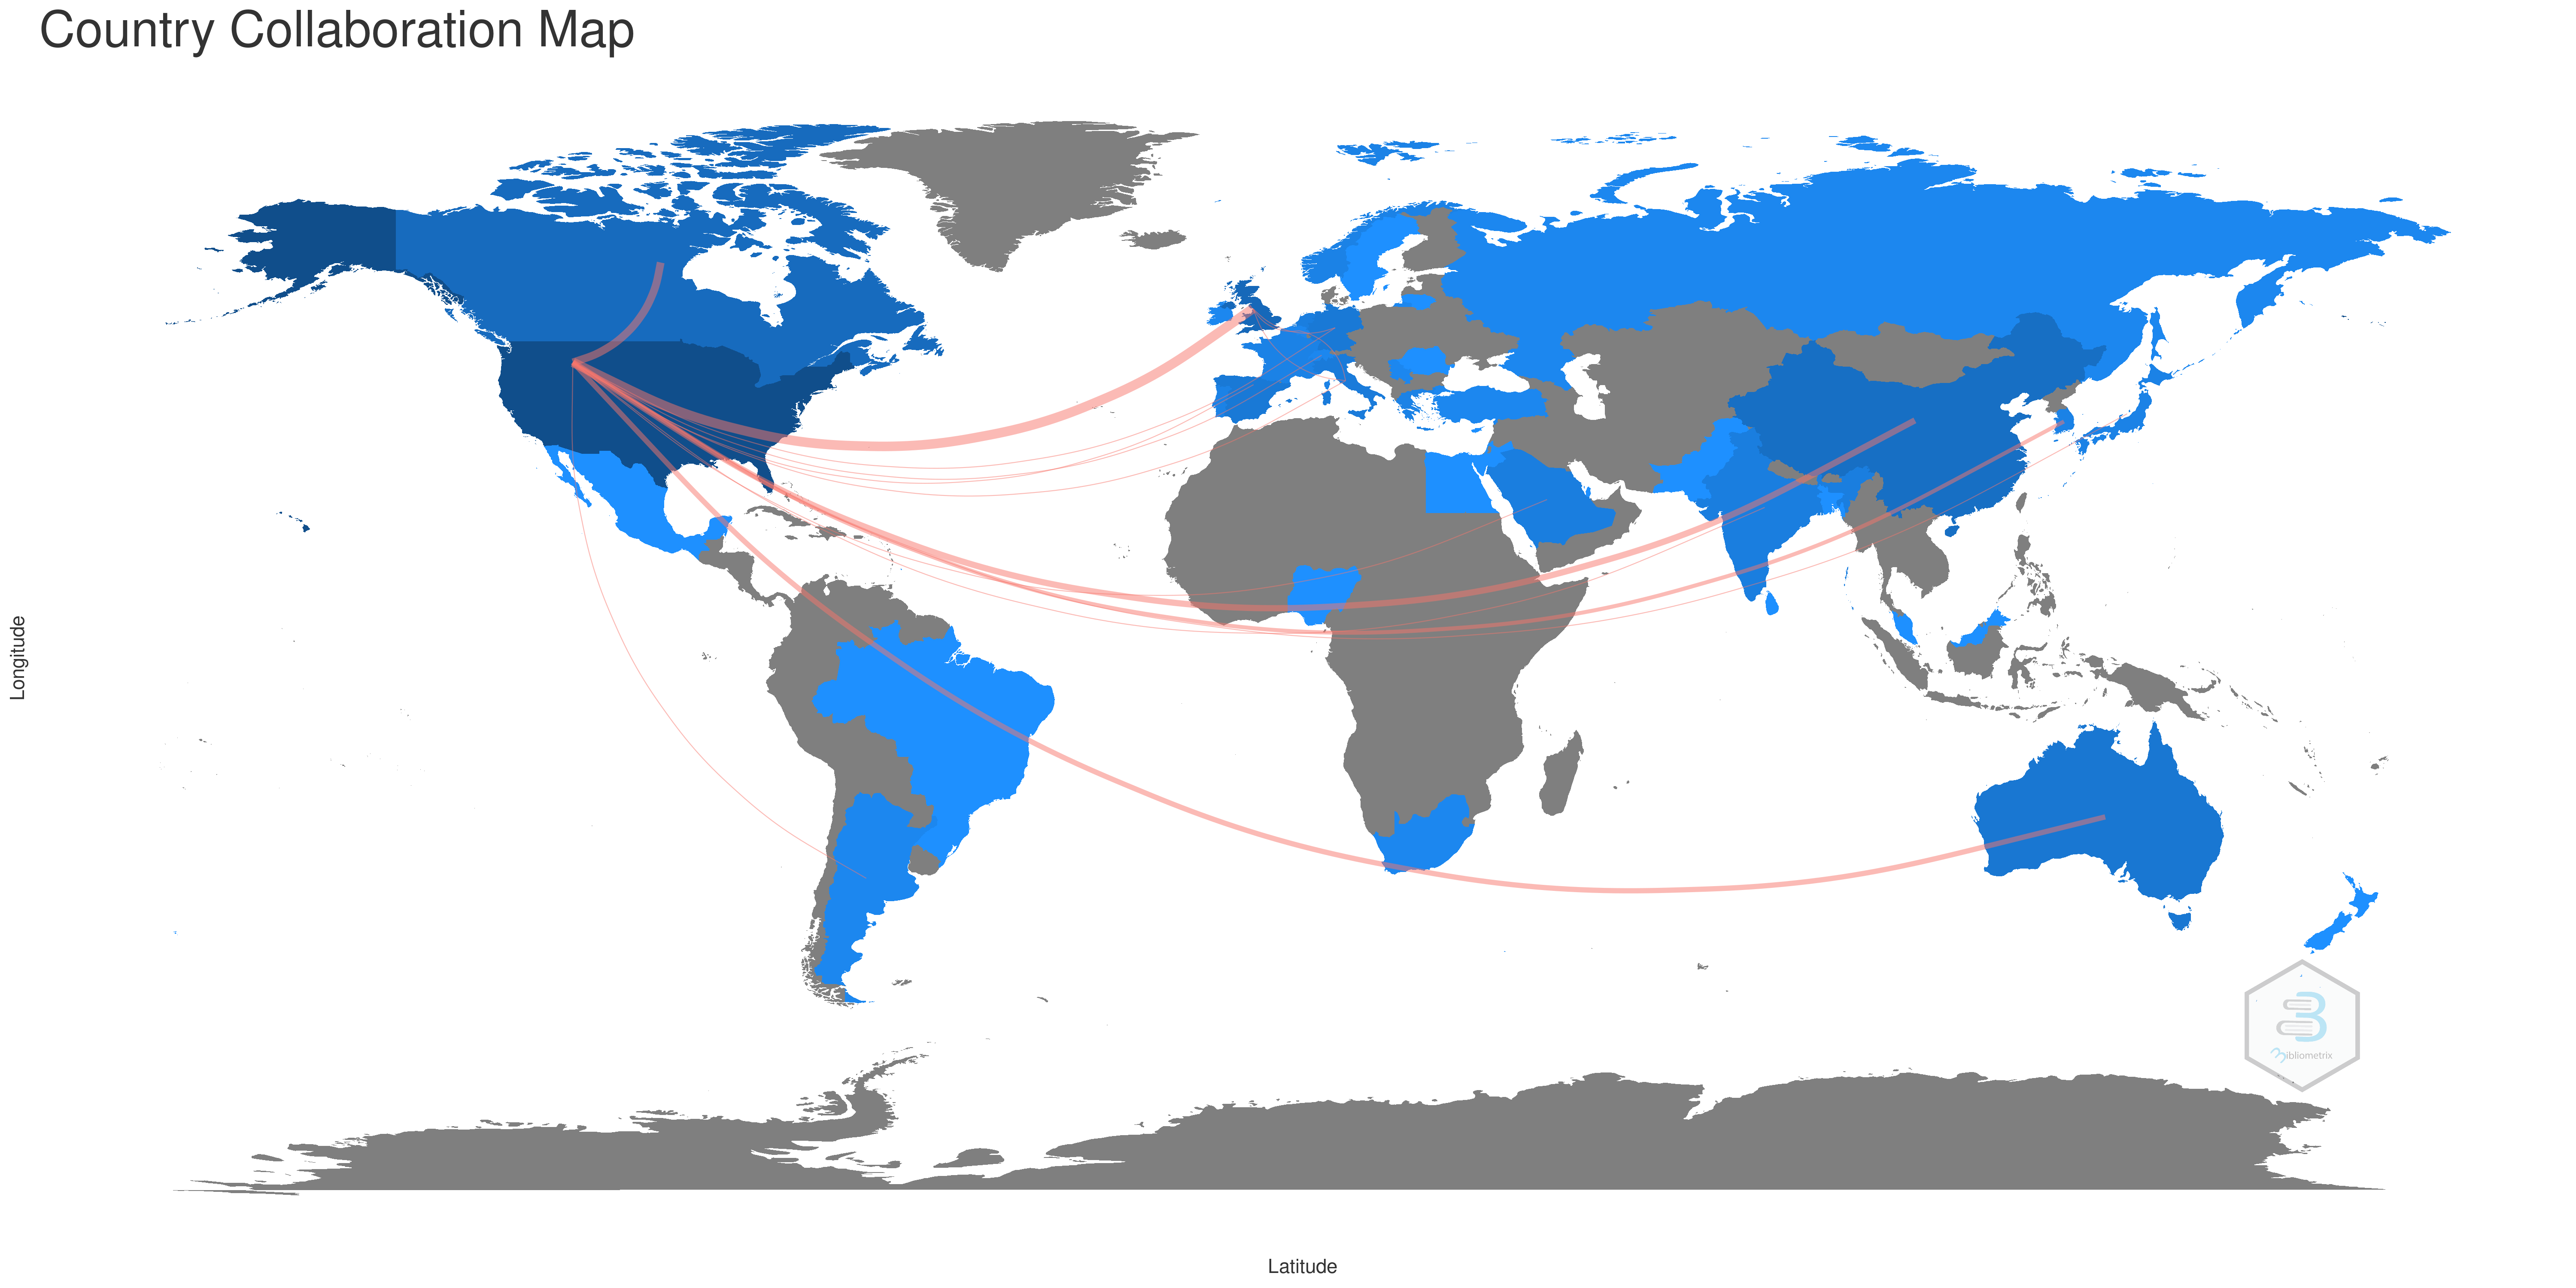
\includegraphics[angle=0,width=1\textwidth]{experiments/ngsylar/PesqBibliogr/Imagens/CountryCollaborationMap-2022-02-09.png}
    \caption{Mapa mundi das Colaborações do dataset ASADES@ngsylar.}
    \label{fig:ASADES@ngsylar:WorldMap}
\end{figure}

Vemos na figura \ref{fig:ASADES@ngsylar:WorldMap}, como as colaborações ocorrem pelo mundo. A imagem está configurada para mostrar vértices os quais possuem no mínimo duas arestas. Entretando, quando aumentamos esse número apenas um pouco, para seis, vemos que a ocorrência das colaborações diminui drásticamente, como mostra a figura \ref{fig:ASADES@ngsylar:WorldMap2}. Ademais, podemos ver que o Estados Unidos concentra a maior parte das colaborações, configurando-se, assim, como um ponto central das colaborações.


\begin{figure}[H]
    \centering
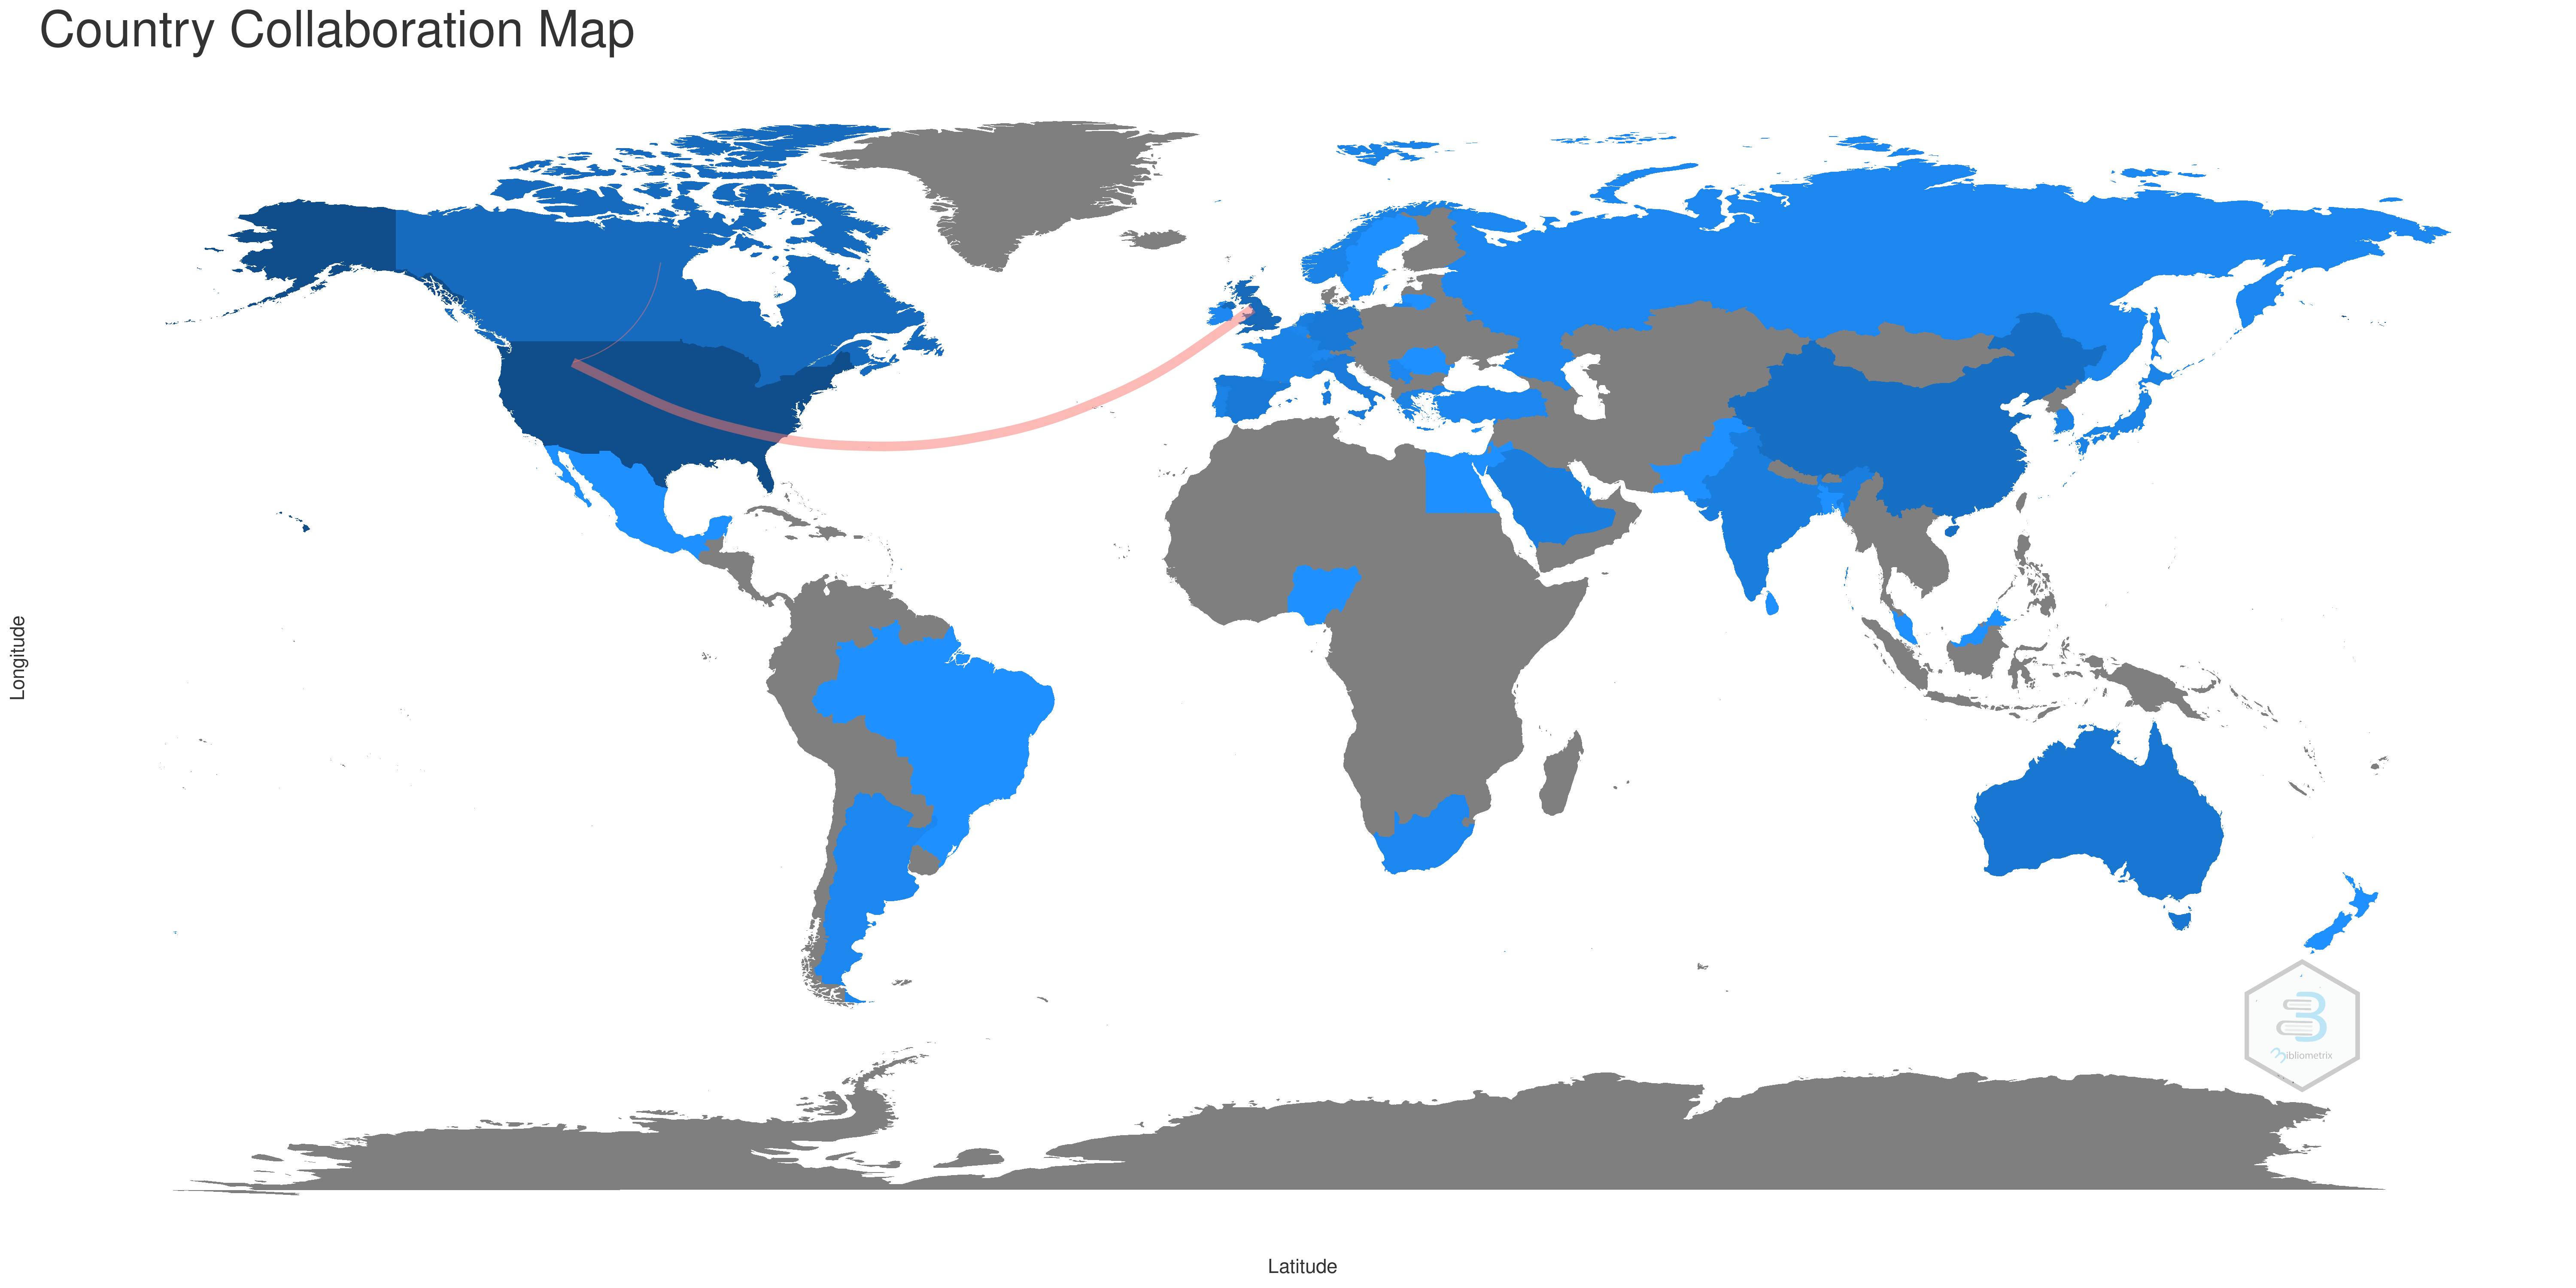
\includegraphics[angle=0,width=1\textwidth]{experiments/ngsylar/PesqBibliogr/Imagens/CountryCollaborationMap-2022-02-09-param6.png}
    \caption{Mapa mundi das Colaborações do dataset ASADES@ngsylar.}
    \label{fig:ASADES@ngsylar:WorldMap2}
\end{figure}

\subsubsection{Rede das Colaborações}

\begin{figure}[H]
    \centering
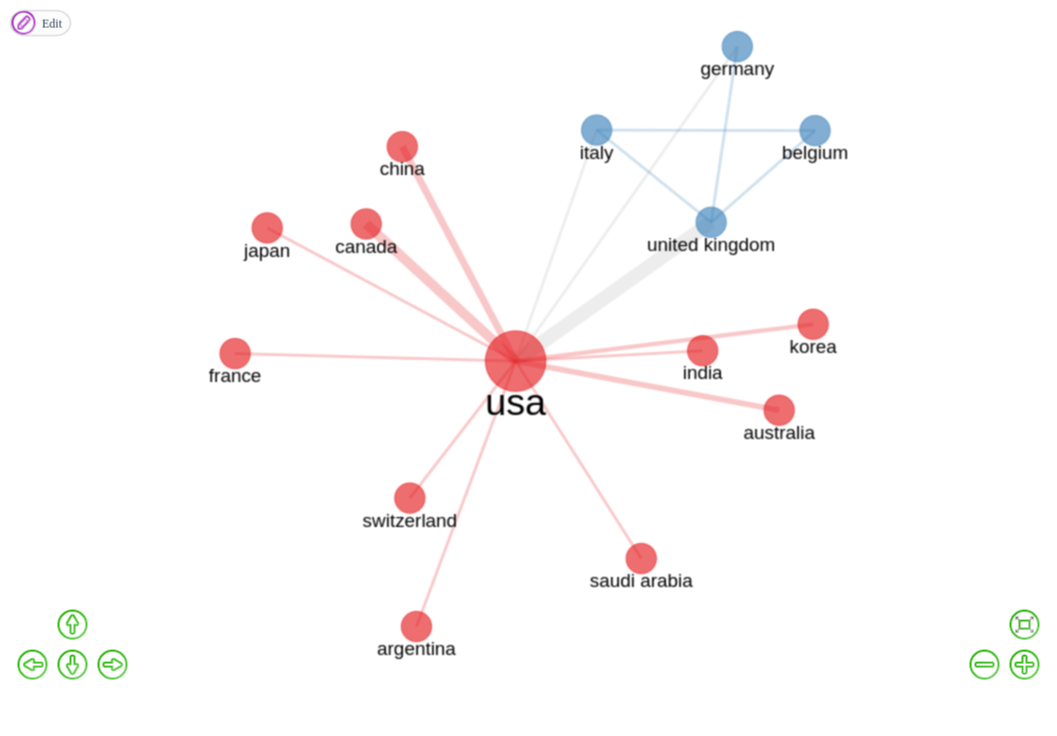
\includegraphics[angle=0,width=1\textwidth]{experiments/ngsylar/PesqBibliogr/Imagens/CollaborationCountries.png}
    \caption{Relações de colaboração entre países do dataset ASADES@ngsylar.}
    \label{fig:ASADES@ngsylar:CollabCountries}
\end{figure}

Na figura \ref{fig:ASADES@ngsylar:WorldMap2}, é possível notar como a interação acerca do tema entre os países é fraca. Temos muitos países que se relacionam unicamente com o Estados Unidos. Portanto, essa imagem, justifica facilmente o porquê das colaborações diminuirem drásticamente no Mapa mundial das Colaborações quando selecionamos o parâmetro mínimo de seis arestas entres os vértices (países). Além do mais, vemos que há duas principais redes de colaboração, uma entre os países da Europa e uma outra, maior e mais significativa, entre os países do mundo com os Estados Unidos. 

\begin{figure}[H]
    \centering
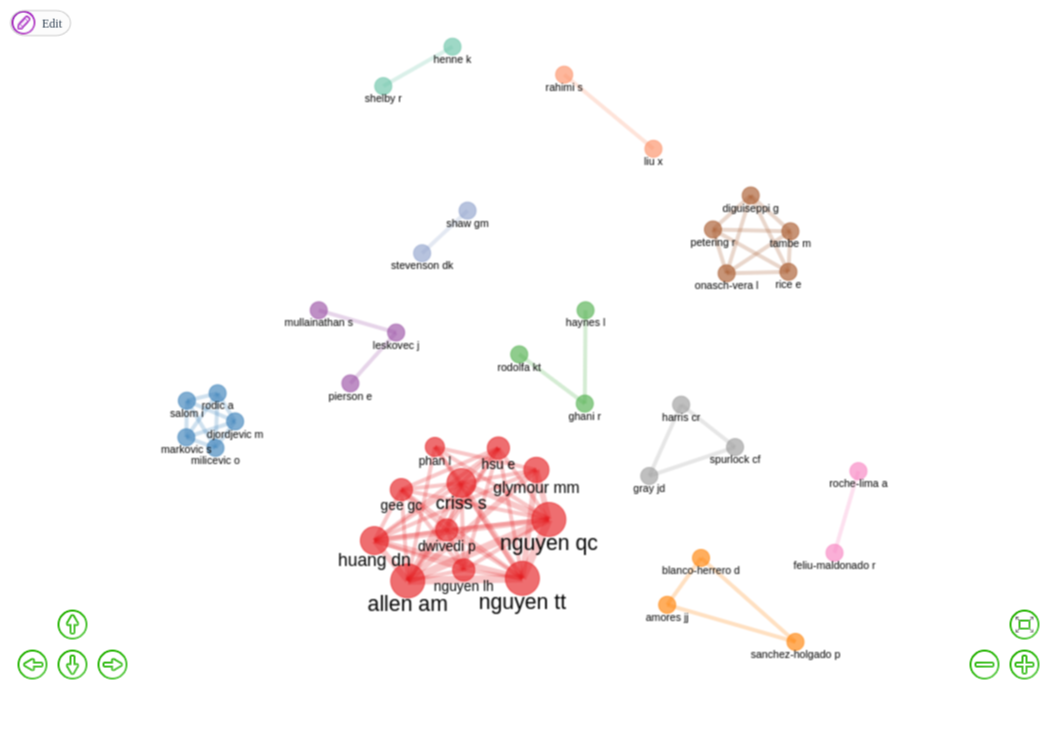
\includegraphics[angle=0,width=1\textwidth]{experiments/ngsylar/PesqBibliogr/Imagens/CollaborationAuthors.png}
    \caption{Relações de colaboração entre Autores do dataset ASADES@ngsylar.}
    \label{fig:ASADES@ngsylar:CollabAuthor}
\end{figure}

\begin{figure}[H]
    \centering
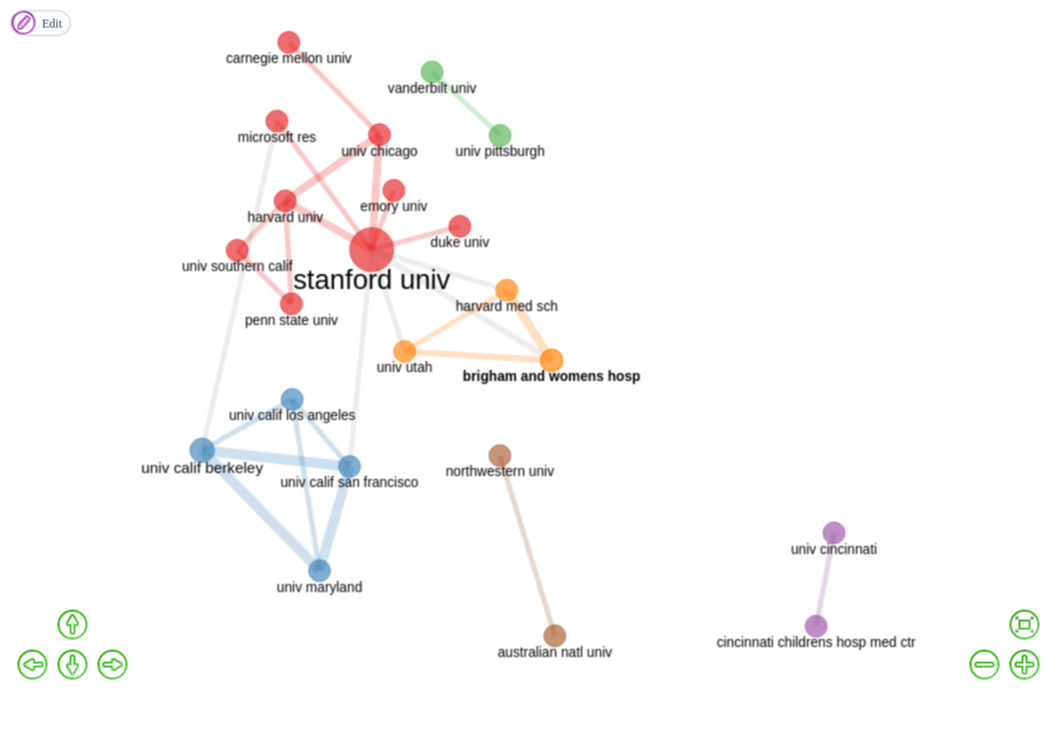
\includegraphics[angle=0,width=1\textwidth]{experiments/ngsylar/PesqBibliogr/Imagens/CollaborationInst.png}
    \caption{Relações de colaboração entre Instituições do dataset ASADES@ngsylar.}
    \label{fig:ASADES@ngsylar:CollabInst}
\end{figure}

Nas figuras \ref{fig:ASADES@ngsylar:CollabAuthor} e \ref{fig:ASADES@ngsylar:CollabInst}, é evidenciado como as relações entre autores e instituições são pouco coesas, são redes fracas, e novamente, ocorre o mesmo comportamento explicitados acima. A colaboração entre autores fica extremamente restrita entre autores de um mesmo grupo, porém aqui observa-se a falta de pelo menos uma conexão que escape o seu grupo e consiga se relacionar com um outro autor de um outro grupo. Consequentemente, o baixo nível do intercâmbio de conhecimentos impacta na qualidade da produção científica mundial. 


Na colaboração entre Instituições, nota-se que as universidades estadunidenses tem maior influência e possui um fluxo maior do intercâmbio do saber científico. E novamente, há grupos os quais ficam totalmente isolados. 

\section{Conclusão}
A criação e disponibilização da \textit{internet} para a população transformou profundamente as relações sociais e culturais com as quais os indivíduos estavam acostumados. Aumentou, também, a dinâmica e volatilidade de como lidamos com tarefas rotineiras, incorporou-se o imediatismo no modo de viver. Aliado a isso, ocorreu também o processo de globalização que utilizou-se da internet para \textit{globalizar} ainda mais o mundo. Dessa forma, foi constituída uma densa rede de comunicação e relacionamento entre países. Com isso, somos impactados com diversas novas informações diariamente, como consequência, na internet, observa-se o fenômeno do \textit{``viral''} --- 